%%%---PREAMBLE---%%%%%%%%%%%%%%%%%%%%%%%%%%%%
\documentclass[twoside,12pt,final]{ucthesis-CA2012}

% fix for pandoc 1.14
\providecommand{\tightlist}{%
  \setlength{\itemsep}{0pt}\setlength{\parskip}{0pt}}

%--- Packages ---------------------------------------------------------
\usepackage[lofdepth,lotdepth,caption=false]{subfig}
\usepackage{fancyhdr}
\usepackage{amsmath, amssymb, graphicx}
\usepackage{xspace}
\usepackage{braket}
\usepackage{color}
\usepackage{setspace}
\usepackage{fancyvrb}
\usepackage{array}
\usepackage{ifxetex,ifluatex}
\usepackage{etoolbox}
\usepackage{booktabs}
\usepackage{xcolor}
\usepackage{tabu}
\usepackage{longtable}
\usepackage{titlesec}
%---New Definitions and Commands------------------------------------------------------

\newtheorem{theorem}{Jibberish}

\bibliography{references}

\hyphenation{mar-gin-al-ia}

% from uw_template.tex

% commands and environments needed by pandoc snippets
% extracted from the output of `pandoc -s`
%% Make R markdown code chunks work

\ifxetex
  \usepackage{fontspec,xltxtra,xunicode}
  \defaultfontfeatures{Mapping=tex-text,Scale=MatchLowercase}
\else
  \ifluatex
    \usepackage{fontspec}
    \defaultfontfeatures{Mapping=tex-text,Scale=MatchLowercase}
  \else
    \usepackage[utf8]{inputenc}
  \fi
\fi
\DefineShortVerb[commandchars=\\\{\}]{\|}
\DefineVerbatimEnvironment{Highlighting}{Verbatim}{commandchars=\\\{\}}
% Add ',fontsize=\small' for more characters per line
\newenvironment{Shaded}{}{}
\newcommand{\KeywordTok}[1]{\textcolor[rgb]{0.00,0.44,0.13}{\textbf{{#1}}}}
\newcommand{\DataTypeTok}[1]{\textcolor[rgb]{0.56,0.13,0.00}{{#1}}}
\newcommand{\DecValTok}[1]{\textcolor[rgb]{0.25,0.63,0.44}{{#1}}}
\newcommand{\BaseNTok}[1]{\textcolor[rgb]{0.25,0.63,0.44}{{#1}}}
\newcommand{\FloatTok}[1]{\textcolor[rgb]{0.25,0.63,0.44}{{#1}}}
\newcommand{\CharTok}[1]{\textcolor[rgb]{0.25,0.44,0.63}{{#1}}}
\newcommand{\StringTok}[1]{\textcolor[rgb]{0.25,0.44,0.63}{{#1}}}
\newcommand{\CommentTok}[1]{\textcolor[rgb]{0.38,0.63,0.69}{\textit{{#1}}}}
\newcommand{\OtherTok}[1]{\textcolor[rgb]{0.00,0.44,0.13}{{#1}}}
\newcommand{\AlertTok}[1]{\textcolor[rgb]{1.00,0.00,0.00}{\textbf{{#1}}}}
\newcommand{\FunctionTok}[1]{\textcolor[rgb]{0.02,0.16,0.49}{{#1}}}
\newcommand{\RegionMarkerTok}[1]{{#1}}
\newcommand{\ErrorTok}[1]{\textcolor[rgb]{1.00,0.00,0.00}{\textbf{{#1}}}}
\newcommand{\NormalTok}[1]{{#1}}
\newcommand{\OperatorTok}[1]{\textcolor[rgb]{0.00,0.44,0.13}{\textbf{{#1}}}}
\newcommand{\BuiltInTok}[1]{\textcolor[rgb]{0.00,0.44,0.13}{\textbf{{#1}}}}
\newcommand{\ControlFlowTok}[1]{\textcolor[rgb]{0.00,0.44,0.13}{\textbf{{#1}}}}

\newlength{\cslhangindent}
\setlength{\cslhangindent}{1.5em}
\newenvironment{cslreferences}%
{\setlength{\parindent}{0pt}%
\everypar{\setlength{\hangindent}{\cslhangindent}}\ignorespaces}%
{\par}

\ifxetex
  \usepackage[setpagesize=false, % page size defined by xetex
              unicode=false, % unicode breaks when used with xetex
              xetex,
              colorlinks=true,
              linkcolor=blue]{hyperref}
\else
  \usepackage[unicode=true,
              colorlinks=true,
              linkcolor=blue]{hyperref}
\fi
\hypersetup{breaklinks=true, pdfborder={0 0 0}}
\setlength{\parindent}{0pt}
\setlength{\parskip}{6pt plus 2pt minus 1pt}
\setlength{\emergencystretch}{3em}  % prevent overfull lines
\setcounter{secnumdepth}{0}

%---Set Margins ------------------------------------------------------
\setlength\oddsidemargin{0.25 in} \setlength\evensidemargin{0.25 in} \setlength\textwidth{6.25 in} \setlength\textheight{8.50 in}
\setlength\footskip{0.25 in} \setlength\topmargin{0 in} \setlength\headheight{0.25 in} \setlength\headsep{0.25 in}

%%%---DOCUMENT---%%%%%%%%%%%%%%%%%%%%%%%%%%%%
\begin{document}

%=== Preliminary Pages ============================================
\begin{ucfrontmatter}

  %%%%%%%%%%%%%%%%%%%%%%%%%%%
  % TITLE PAGE INFORMATION %
  %%%%%%%%%%%%%%%%%%%%%%%%%%%

  \title{Improving the Management of Marine Resources through Economics and Data Science}

  \author{Joshua Johnson}

  \report{Dissertation} \degree{Doctor of Philosophy} \degreemonth{June} \degreeyear{2018}
  \defensemonth{May}
  \defenseyear{2018}

  \chair{Professor Christopher Costello}  % this is your advisor
  \othermemberA{Professor Steven Gaines} % This is a member of your committee
  \othermemberB{Professor Ray Hilborn} % This is a member of your committee
  \othermemberC{Professor Olivier Deschenes} % This is a member of your committee (if your department requires 4 members)
  \numberofmembers{4} % should match the number of entries above (chair + othermembers)

  \field{Slowly and Painfully Working Out the Surprisingly Obvious}
  \campus{Santa Barbara}
	\maketitle
	\approvalpage
	\copyrightpage

  %%%%%%%%%%%%%%%%%%%%%%%%%%%
  % DEDICATION PAGE INFORMATION %
  %%%%%%%%%%%%%%%%%%%%%%%%%%%
    \begin{dedication}

      \vspace*{25ex}
      \begin{center}
      \begin{Large}

        To Hobbes

      \end{Large}
      \end{center}
  \end{dedication}
  \begin{acknowledgements}
    Thanks everyone!
  \end{acknowledgements}
	%%%%%%%%%%%%%%%%%%%%%%%%%%%
  % ABSTRACT %
  %%%%%%%%%%%%%%%%%%%%%%%%%%%
  \begin{abstract}
    \addcontentsline{toc}{chapter}{Abstract}
    %todo: max 350 words

    The data say `meh'

    %\abstractsignature
  \end{abstract}
	\tableofcontents

	  \listoftables
  
    \listoffigures
  
\end{ucfrontmatter}
\begin{ucmainmatter}

\hypertarget{intro}{%
\chapter{Introduction}\label{intro}}

Welcome to the \emph{R Markdown} thesis template. This template is based on (and in many places copied directly from) the UW LaTeX template, but hopefully it will provide a nicer interface for those that have never used TeX or LaTeX before. Using \emph{R Markdown} will also allow you to easily keep track of your analyses in \textbf{R} chunks of code, with the resulting plots and output included as well. The hope is this \emph{R Markdown} template gets you in the habit of doing reproducible research, which benefits you long-term as a researcher, but also will greatly help anyone that is trying to reproduce or build onto your results down the road.

Hopefully, you won't have much of a learning period to go through and you will reap the benefits of a nicely formatted thesis. The use of LaTeX in combination with \emph{Markdown} is more consistent than the output of a word processor, much less prone to corruption or crashing, and the resulting file is smaller than a Word file. While you may have never had problems using Word in the past, your thesis is likely going to be at least twice as large and complex as anything you've written before, taxing Word's capabilities. After working with \emph{Markdown} and \textbf{R} together for a few weeks, we are confident this will be your reporting style of choice going forward.

\textbf{Why use it?}

\emph{R Markdown} creates a simple and straightforward way to interface with the beauty of LaTeX. Packages have been written in \textbf{R} to work directly with LaTeX to produce nicely formatting tables and paragraphs. In addition to creating a user friendly interface to LaTeX, \emph{R Markdown} also allows you to read in your data, to analyze it and to visualize it using \textbf{R} functions, and also to provide the documentation and commentary on the results of your project. Further, it allows for \textbf{R} results to be passed inline to the commentary of your results. You'll see more on this later.

\textbf{Who should use it?}

Anyone who needs to use data analysis, math, tables, a lot of figures, complex cross-references, or who just cares about the final appearance of their document should use \emph{R Markdown}. Of particular use should be anyone in the sciences, but the user-friendly nature of \emph{Markdown} and its ability to keep track of and easily include figures, automatically generate a table of contents, index, references, table of figures, etc. should make it of great benefit to nearly anyone writing a thesis project.

\hypertarget{rmd-basics}{%
\chapter{R Markdown Basics}\label{rmd-basics}}

\chaptermark{Basics}

Here is a brief introduction into using \emph{R Markdown}. \emph{Markdown} is a simple formatting syntax for authoring HTML, PDF, and MS Word documents. \emph{R Markdown} provides the flexibility of \emph{Markdown} with the implementation of \textbf{R} input and output. For more details on using \emph{R Markdown} see \url{http://rmarkdown.rstudio.com}.

Be careful with your spacing in \emph{Markdown} documents. While whitespace largely is ignored, it does at times give \emph{Markdown} signals as to how to proceed. As a habit, try to keep everything left aligned whenever possible, especially as you type a new paragraph. In other words, there is no need to indent basic text in the Rmd document (in fact, it might cause your text to do funny things if you do).

\hypertarget{lists}{%
\section{Lists}\label{lists}}

It's easy to create a list. It can be unordered like
\begin{itemize}
\tightlist
\item
  Item 1
\item
  Item 2
\end{itemize}
or it can be ordered like
\begin{enumerate}
\def\labelenumi{\arabic{enumi}.}
\tightlist
\item
  Item 1
\item
  Item 2
\end{enumerate}
Notice that I intentionally mislabeled Item 2 as number 4. \emph{Markdown} automatically figures this out! You can put any numbers in the list and it will create the list. Check it out below.

To create a sublist, just indent the values a bit (at least four spaces or a tab). (Here's one case where indentation is key!)
\begin{enumerate}
\def\labelenumi{\arabic{enumi}.}
\tightlist
\item
  Item 1
\item
  Item 2
\item
  Item 3
  \begin{itemize}
  \tightlist
  \item
    Item 3a
  \item
    Item 3b
  \end{itemize}
\end{enumerate}
\hypertarget{line-breaks}{%
\section{Line breaks}\label{line-breaks}}

Make sure to add white space between lines if you'd like to start a new paragraph. Look at what happens below in the outputted document if you don't:

Here is the first sentence. Here is another sentence. Here is the last sentence to end the paragraph.
This should be a new paragraph.

\emph{Now for the correct way:}

Here is the first sentence. Here is another sentence. Here is the last sentence to end the paragraph.

This should be a new paragraph.

\hypertarget{r-chunks}{%
\section{R chunks}\label{r-chunks}}

When you click the \textbf{Knit} button above a document will be generated that includes both content as well as the output of any embedded \textbf{R} code chunks within the document. You can embed an \textbf{R} code chunk like this (\texttt{cars} is a built-in \textbf{R} dataset):
\begin{Shaded}
\begin{Highlighting}[]
\KeywordTok{summary}\NormalTok{(cars)}
\end{Highlighting}
\end{Shaded}
\begin{verbatim}
     speed           dist       
 Min.   : 4.0   Min.   :  2.00  
 1st Qu.:12.0   1st Qu.: 26.00  
 Median :15.0   Median : 36.00  
 Mean   :15.4   Mean   : 42.98  
 3rd Qu.:19.0   3rd Qu.: 56.00  
 Max.   :25.0   Max.   :120.00  
\end{verbatim}
\hypertarget{inline-code}{%
\section{Inline code}\label{inline-code}}

If you'd like to put the results of your analysis directly into your discussion, add inline code like this:
\begin{quote}
The \texttt{cos} of \(2 \pi\) is 1.
\end{quote}
Another example would be the direct calculation of the standard deviation:
\begin{quote}
The standard deviation of \texttt{speed} in \texttt{cars} is 5.2876444.
\end{quote}
One last neat feature is the use of the \texttt{ifelse} conditional statement which can be used to output text depending on the result of an \textbf{R} calculation:
\begin{quote}
The standard deviation is less than 6.
\end{quote}
Note the use of \texttt{\textgreater{}} here, which signifies a quotation environment that will be indented.

As you see with \texttt{\$2\ \textbackslash{}pi\$} above, mathematics can be added by surrounding the mathematical text with dollar signs. More examples of this are in {[}Mathematics and Science{]} if you uncomment the code in \protect\hyperlink{math}{Math}.

\hypertarget{including-plots}{%
\section{Including plots}\label{including-plots}}

You can also embed plots. For example, here is a way to use the base \textbf{R} graphics package to produce a plot using the built-in \texttt{pressure} dataset:

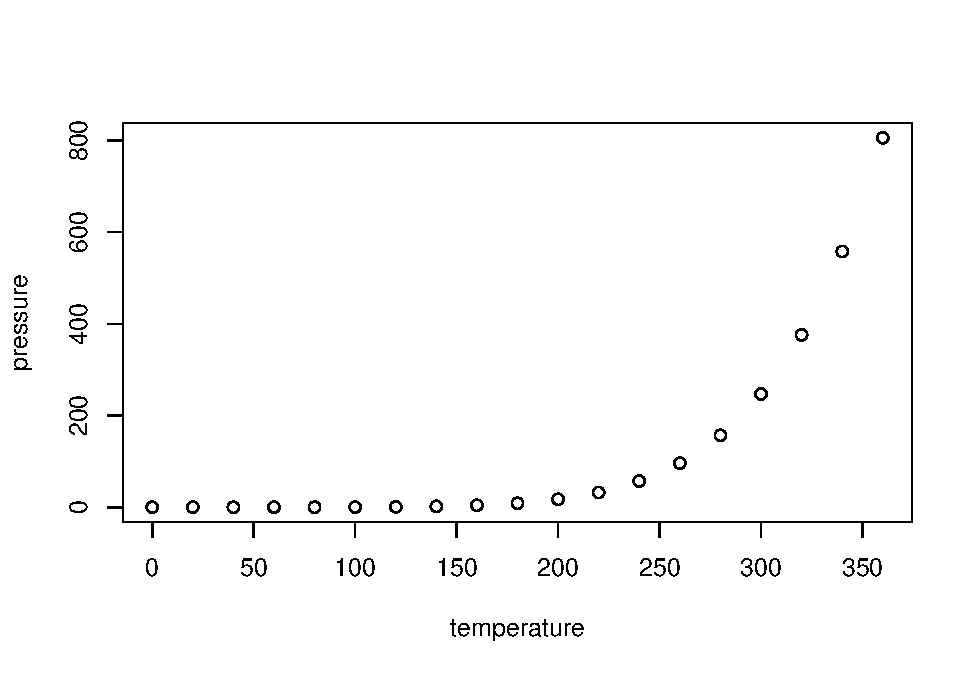
\includegraphics{thesis2_files/figure-latex/pressure-1.pdf}

Note that the \texttt{echo=FALSE} parameter was added to the code chunk to prevent printing of the \textbf{R} code that generated the plot. There are plenty of other ways to add chunk options. More information is available at \url{http://yihui.name/knitr/options/}.

Another useful chunk option is the setting of \texttt{cache=TRUE} as you see here. If document rendering becomes time consuming due to long computations or plots that are expensive to generate you can use knitr caching to improve performance. Later in this file, you'll see a way to reference plots created in \textbf{R} or external figures.

\hypertarget{loading-and-exploring-data}{%
\section{Loading and exploring data}\label{loading-and-exploring-data}}

Included in this template is a file called \texttt{flights.csv}. This file includes a subset of the larger dataset of information about all flights that departed from Seattle and Portland in 2014. More information about this dataset and its \textbf{R} package is available at \url{http://github.com/ismayc/pnwflights14}. This subset includes only Portland flights and only rows that were complete with no missing values. Merges were also done with the \texttt{airports} and \texttt{airlines} data sets in the \texttt{pnwflights14} package to get more descriptive airport and airline names.

We can load in this data set using the following command:
\begin{Shaded}
\begin{Highlighting}[]
\NormalTok{flights <-}\StringTok{ }\KeywordTok{read.csv}\NormalTok{(}\StringTok{"data/flights.csv"}\NormalTok{)}
\end{Highlighting}
\end{Shaded}
The data is now stored in the data frame called \texttt{flights} in \textbf{R}. To get a better feel for the variables included in this dataset we can use a variety of functions. Here we can see the dimensions (rows by columns) and also the names of the columns.
\begin{Shaded}
\begin{Highlighting}[]
\KeywordTok{dim}\NormalTok{(flights)}
\end{Highlighting}
\end{Shaded}
\begin{verbatim}
[1] 52808    16
\end{verbatim}
\begin{Shaded}
\begin{Highlighting}[]
\KeywordTok{names}\NormalTok{(flights)}
\end{Highlighting}
\end{Shaded}
\begin{verbatim}
 [1] "month"        "day"          "dep_time"     "dep_delay"    "arr_time"    
 [6] "arr_delay"    "carrier"      "tailnum"      "flight"       "dest"        
[11] "air_time"     "distance"     "hour"         "minute"       "carrier_name"
[16] "dest_name"   
\end{verbatim}
Another good idea is to take a look at the dataset in table form. With this dataset having more than 50,000 rows, we won't explicitly show the results of the command here. I recommend you enter the command into the Console \textbf{\emph{after}} you have run the \textbf{R} chunks above to load the data into \textbf{R}.
\begin{Shaded}
\begin{Highlighting}[]
\KeywordTok{View}\NormalTok{(flights)}
\end{Highlighting}
\end{Shaded}
While not required, it is highly recommended you use the \texttt{dplyr} package to manipulate and summarize your data set as needed. It uses a syntax that is easy to understand using chaining operations. Below I've created a few examples of using \texttt{dplyr} to get information about the Portland flights in 2014. You will also see the use of the \texttt{ggplot2} package, which produces beautiful, high-quality academic visuals.

We begin by checking to ensure that needed packages are installed and then we load them into our current working environment:
\begin{Shaded}
\begin{Highlighting}[]
\CommentTok{# List of packages required for this analysis}
\NormalTok{pkg <-}\StringTok{ }\KeywordTok{c}\NormalTok{(}\StringTok{"dplyr"}\NormalTok{, }\StringTok{"ggplot2"}\NormalTok{, }\StringTok{"knitr"}\NormalTok{, }\StringTok{"bookdown"}\NormalTok{, }\StringTok{"devtools"}\NormalTok{)}
\CommentTok{# Check if packages are not installed and assign the}
\CommentTok{# names of the packages not installed to the variable new.pkg}
\NormalTok{new.pkg <-}\StringTok{ }\NormalTok{pkg[}\OperatorTok{!}\NormalTok{(pkg }\OperatorTok\StringTok{ }\KeywordTok{installed.packages}\NormalTok{())]}
\CommentTok{# If there are any packages in the list that aren't installed,}
\CommentTok{# install them}
\ControlFlowTok{if}\NormalTok{ (}\KeywordTok{length}\NormalTok{(new.pkg))}
  \KeywordTok{install.packages}\NormalTok{(new.pkg, }\DataTypeTok{repos =} \StringTok{"http://cran.rstudio.com"}\NormalTok{)}
\CommentTok{# Load packages (huskydown will load all of the packages as well)}
\KeywordTok{library}\NormalTok{(gauchodown)}
\end{Highlighting}
\end{Shaded}
\clearpage

The example we show here does the following:
\begin{itemize}
\item
  Selects only the \texttt{carrier\_name} and \texttt{arr\_delay} from the \texttt{flights} dataset and then assigns this subset to a new variable called \texttt{flights2}.
\item
  Using \texttt{flights2}, we determine the largest arrival delay for each of the carriers.
\end{itemize}
\begin{Shaded}
\begin{Highlighting}[]
\KeywordTok{library}\NormalTok{(dplyr)}
\end{Highlighting}
\end{Shaded}
\begin{verbatim}

Attaching package: 'dplyr'
\end{verbatim}
\begin{verbatim}
The following objects are masked from 'package:stats':

    filter, lag
\end{verbatim}
\begin{verbatim}
The following objects are masked from 'package:base':

    intersect, setdiff, setequal, union
\end{verbatim}
\begin{Shaded}
\begin{Highlighting}[]
\NormalTok{flights2 <-}\StringTok{ }\NormalTok{flights }\OperatorTok\StringTok{ }
\StringTok{  }\KeywordTok{select}\NormalTok{(carrier_name, arr_delay)}
\NormalTok{max_delays <-}\StringTok{ }\NormalTok{flights2 }\OperatorTok\StringTok{ }
\StringTok{  }\KeywordTok{group_by}\NormalTok{(carrier_name) }\OperatorTok
\StringTok{  }\KeywordTok{summarize}\NormalTok{(}\DataTypeTok{max_arr_delay =} \KeywordTok{max}\NormalTok{(arr_delay, }\DataTypeTok{na.rm =} \OtherTok{TRUE}\NormalTok{))}
\end{Highlighting}
\end{Shaded}
\begin{verbatim}
`summarise()` ungrouping output (override with `.groups` argument)
\end{verbatim}
A useful function in the \texttt{knitr} package for making nice tables in \emph{R Markdown} is called \texttt{kable}. It is much easier to use than manually entering values into a table by copying and pasting values into Excel or LaTeX. This again goes to show how nice reproducible documents can be! (Note the use of \texttt{results="asis"}, which will produce the table instead of the code to create the table.) The \texttt{caption.short} argument is used to include a shorter title to appear in the List of Tables.
\begin{Shaded}
\begin{Highlighting}[]
\KeywordTok{library}\NormalTok{(knitr)}
\KeywordTok{kable}\NormalTok{(max_delays, }
      \DataTypeTok{col.names =} \KeywordTok{c}\NormalTok{(}\StringTok{"Airline"}\NormalTok{, }\StringTok{"Max Arrival Delay"}\NormalTok{),}
      \DataTypeTok{caption =} \StringTok{"Maximum Delays by Airline"}\NormalTok{,}
      \DataTypeTok{caption.short =} \StringTok{"Max Delays by Airline"}\NormalTok{,}
      \DataTypeTok{longtable =} \OtherTok{TRUE}\NormalTok{,}
      \DataTypeTok{booktabs =} \OtherTok{TRUE}\NormalTok{)}
\end{Highlighting}
\end{Shaded}
\begin{longtable}[t]{lr}
\caption[Max Delays by Airline]{\label{tab:maxdelays}Maximum Delays by Airline}\\
\toprule
Airline & Max Arrival Delay\\
\midrule
Alaska Airlines Inc. & 338\\
American Airlines Inc. & 1539\\
Delta Air Lines Inc. & 651\\
Frontier Airlines Inc. & 575\\
Hawaiian Airlines Inc. & 407\\
\addlinespace
JetBlue Airways & 273\\
SkyWest Airlines Inc. & 421\\
Southwest Airlines Co. & 694\\
United Air Lines Inc. & 472\\
US Airways Inc. & 347\\
\addlinespace
Virgin America & 366\\
\bottomrule
\end{longtable}
The last two options make the table a little easier-to-read.

We can further look into the properties of the largest value here for American Airlines Inc.~To do so, we can isolate the row corresponding to the arrival delay of 1539 minutes for American in our original \texttt{flights} dataset.
\begin{Shaded}
\begin{Highlighting}[]
\NormalTok{flights }\OperatorTok\StringTok{ }
\StringTok{  }\KeywordTok{filter}\NormalTok{(arr_delay }\OperatorTok{==}\StringTok{ }\DecValTok{1539}\NormalTok{, }
\NormalTok{         carrier_name }\OperatorTok{==}\StringTok{ "American Airlines Inc."}\NormalTok{) }\OperatorTok
\StringTok{  }\KeywordTok{select}\NormalTok{(}\OperatorTok{-}\KeywordTok{c}\NormalTok{(month, day, carrier, dest_name, hour, }
\NormalTok{            minute, carrier_name, arr_delay))}
\end{Highlighting}
\end{Shaded}
\begin{verbatim}
  dep_time dep_delay arr_time tailnum flight dest air_time distance
1     1403      1553     1934  N595AA   1568  DFW      182     1616
\end{verbatim}
We see that the flight occurred on March 3rd and departed a little after 2 PM on its way to Dallas/Fort Worth. Lastly, we show how we can visualize the arrival delay of all departing flights from Portland on March 3rd against time of departure.
\begin{Shaded}
\begin{Highlighting}[]
\KeywordTok{library}\NormalTok{(ggplot2)}
\NormalTok{flights }\OperatorTok\StringTok{ }
\StringTok{  }\KeywordTok{filter}\NormalTok{(month }\OperatorTok{==}\StringTok{ }\DecValTok{3}\NormalTok{, day }\OperatorTok{==}\StringTok{ }\DecValTok{3}\NormalTok{) }\OperatorTok
\StringTok{  }\KeywordTok{ggplot}\NormalTok{(}\KeywordTok{aes}\NormalTok{(}\DataTypeTok{x =}\NormalTok{ dep_time, }
             \DataTypeTok{y =}\NormalTok{ arr_delay)) }\OperatorTok{+}\StringTok{ }
\StringTok{  }\KeywordTok{geom_point}\NormalTok{()}
\end{Highlighting}
\end{Shaded}
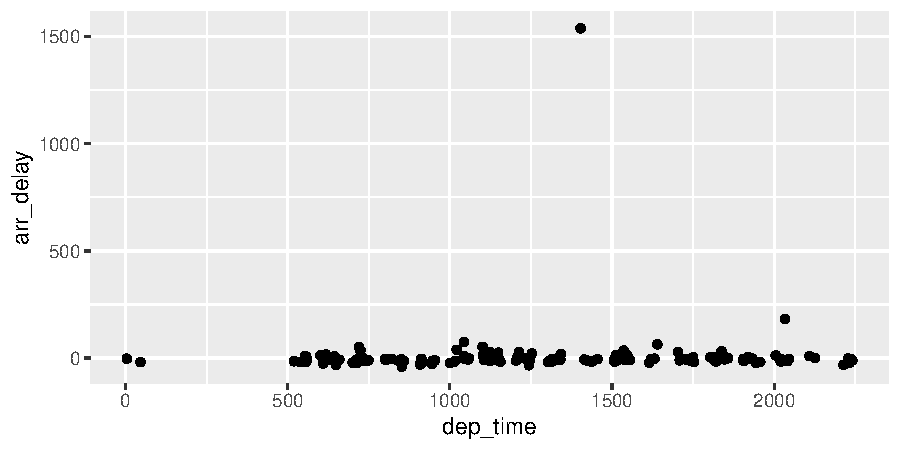
\includegraphics{thesis2_files/figure-latex/march3plot-1.pdf}

\hypertarget{additional-resources}{%
\section{Additional resources}\label{additional-resources}}
\begin{itemize}
\item
  \emph{Markdown} Cheatsheet - \url{https://github.com/adam-p/markdown-here/wiki/Markdown-Cheatsheet}
\item
  \emph{R Markdown} Reference Guide - \url{https://www.rstudio.com/wp-content/uploads/2015/03/rmarkdown-reference.pdf}
\item
  Introduction to \texttt{dplyr} - \url{https://cran.rstudio.com/web/packages/dplyr/vignettes/introduction.html}
\item
  \texttt{ggplot2} Documentation - \url{http://docs.ggplot2.org/current/}
\end{itemize}
\hypertarget{math-sci}{%
\chapter{Results}\label{math-sci}}

\hypertarget{packages-data-loading-etc.}{%
\chapter{Packages, data loading etc.}\label{packages-data-loading-etc.}}
\begin{Shaded}
\begin{Highlighting}[]
\KeywordTok{library}\NormalTok{(tidyverse)}
\KeywordTok{library}\NormalTok{(dplyr)}
\KeywordTok{library}\NormalTok{(ggplot2)}
\KeywordTok{library}\NormalTok{(cowplot)}
\KeywordTok{library}\NormalTok{(reshape2)}
\KeywordTok{library}\NormalTok{(rstatix)}
\KeywordTok{library}\NormalTok{(ggpubr)}
\KeywordTok{library}\NormalTok{(nlme)}
\KeywordTok{library}\NormalTok{(lme4)}
\end{Highlighting}
\end{Shaded}
\hypertarget{basic-statistics-and-data-mangling}{%
\chapter{Basic statistics and data mangling}\label{basic-statistics-and-data-mangling}}
\begin{verbatim}
# A tibble: 80 x 5
   type  id        n avg.qty sd.qty
   <chr> <fct> <int>   <dbl>  <dbl>
 1 rhizo 198       3 230588. 12686.
 2 rhizo 201       3 228907.  6576.
 3 rhizo 206       3 332463.  6923.
 4 rhizo 212       3 210821. 25403.
 5 rhizo 216       3 488172. 25382.
 6 rhizo 224       3 252674. 30488.
 7 rhizo 226       3 353033. 31415.
 8 rhizo 232       3 583033. 12524.
 9 rhizo 234       3 522109. 92493.
10 rhizo 237       3 287493.  3463.
# ... with 70 more rows
\end{verbatim}
\begin{verbatim}
# A tibble: 80 x 10
   type  id        n avg.qty sd.qty dna_conc unit      qty_undil   qty_ul qty_ng
   <chr> <fct> <int>   <dbl>  <dbl>    <dbl> <chr>         <dbl>    <dbl>  <dbl>
 1 rhizo 198       3 230588. 12686.     35.8 DNA[ng_~  92235246.   1.15e7 3.22e5
 2 rhizo 201       3 228907.  6576.     38.1 DNA[ng_~  91562808.   1.14e7 3.00e5
 3 rhizo 206       3 332463.  6923.     47.5 DNA[ng_~ 132985071.   1.66e7 3.50e5
 4 rhizo 212       3 210821. 25403.     35.1 DNA[ng_~  84328527.   1.05e7 3.01e5
 5 rhizo 216       3 488172. 25382.     52.8 DNA[ng_~ 195268783.   2.44e7 4.62e5
 6 rhizo 224       3 252674. 30488.     38.6 DNA[ng_~ 101069454.   1.26e7 3.27e5
 7 rhizo 226       3 353033. 31415.     50.3 DNA[ng_~ 141213354.   1.77e7 3.51e5
 8 rhizo 232       3 583033. 12524.     60.2 DNA[ng_~ 233213183.   2.92e7 4.85e5
 9 rhizo 234       3 522109. 92493.     61.1 DNA[ng_~ 208843525    2.61e7 4.27e5
10 rhizo 237       3 287493.  3463.     43.1 DNA[ng_~ 114997088.   1.44e7 3.34e5
# ... with 70 more rows
\end{verbatim}
\begin{verbatim}
# A tibble: 80 x 11
   type  id     qty_ng unit      treatment fert  fung  block row   time  subject
   <chr> <fct>   <dbl> <chr>     <chr>     <fct> <fct> <fct> <fct> <fct>   <dbl>
 1 rhizo 198   321871. GeneCopi~ H00       no    no    b     1     t2          1
 2 rhizo 201   300167. GeneCopi~ H00       no    no    c     1     t2          2
 3 rhizo 206   350108. GeneCopi~ H01       yes   no    b     1     t2          6
 4 rhizo 212   300572. GeneCopi~ HP0       no    yes   b     1     t2         11
 5 rhizo 216   462284. GeneCopi~ HP1       yes   yes   b     1     t2         16
 6 rhizo 224   327467. GeneCopi~ HP0       no    yes   c     2     t2         12
 7 rhizo 226   350719. GeneCopi~ HP0       no    yes   e     2     t2         13
 8 rhizo 232   484569. GeneCopi~ H00       no    no    d     2     t2          3
 9 rhizo 234   427258. GeneCopi~ HP1       yes   yes   c     2     t2         17
10 rhizo 237   333828. GeneCopi~ H01       yes   no    c     2     t2          7
# ... with 70 more rows
\end{verbatim}
The data preparation is finished for the 16s rRNA gene copy data. We have worked with the raw quantity values used qPCR machine (standardized on the individual runs standard curve), did summary statistics (averaging the technical replicates) and calculated gene copy number per nanogram DNA.

Now we move on to the statistical modelling and checking for significance.

\hypertarget{statistical-modelling-and-sig.-testing}{%
\chapter{Statistical modelling and sig. testing}\label{statistical-modelling-and-sig.-testing}}

\hypertarget{rhizo}{%
\section{Rhizo}\label{rhizo}}

\hypertarget{checking-data-balance}{%
\subsection{Checking data balance}\label{checking-data-balance}}
\begin{verbatim}
# A tibble: 8 x 7
  fert  fung  time  variable     n    mean     sd
  <fct> <fct> <fct> <chr>    <dbl>   <dbl>  <dbl>
1 no    no    t2    qty_ng       5 371209. 74345.
2 no    no    t3    qty_ng       5 240046. 28114.
3 no    yes   t2    qty_ng       5 333985. 22320.
4 no    yes   t3    qty_ng       5 259493. 16454.
5 yes   no    t2    qty_ng       5 335729. 19108.
6 yes   no    t3    qty_ng       5 300139. 64159.
7 yes   yes   t2    qty_ng       5 406397. 52670.
8 yes   yes   t3    qty_ng       5 297449. 24004.
\end{verbatim}
We have a balanced dataset (n is the same for each group). Moving on to a boxplot to visually inspect groups and look for outliers.

\includegraphics{thesis2_files/figure-latex/rhizo 16s boxplots-1.pdf}

We have one outlier in {[}fert:no\textbar fung:no\textbar time:t3{]} and two outliers in {[}fert:yes\textbar fung:yes\textbar time:t2{]}. Identifying the outliers:
\begin{verbatim}
# A tibble: 3 x 10
  fert  fung  time  id     qty_ng block row   subject is.outlier is.extreme
  <fct> <fct> <fct> <fct>   <dbl> <fct> <fct>   <dbl> <lgl>      <lgl>     
1 no    no    t3    355   290010. e     3           4 TRUE       TRUE      
2 yes   yes   t2    216   462284. b     1          16 TRUE       FALSE     
3 yes   yes   t2    253   319869. f     3          18 TRUE       TRUE      
\end{verbatim}
Replicate 216, 355 and 253 are outliers. The two last ones are extreme outliers. Consult the `index' file to see the differences between the replicates and their respective groups.
\begin{quote}
Values above Q3 + 1.5xIQR or below Q1 - 1.5xIQR are considered as outliers. Values above Q3 + 3xIQR or below Q1 - 3xIQR are considered as extreme points (or extreme outliers).
\end{quote}
We will perform the following analysis with and without the extreme outliers.

\hypertarget{normality-and-heteroskedasticity}{%
\subsection{Normality and heteroskedasticity}\label{normality-and-heteroskedasticity}}
\begin{Shaded}
\begin{Highlighting}[]
  \CommentTok{# Normality test with all outliers (Shapiro Test)}
    
\NormalTok{  genecopy.work }\OperatorTok
\StringTok{    }\KeywordTok{group_by}\NormalTok{(fert, fung, time) }\OperatorTok
\StringTok{    }\KeywordTok{shapiro_test}\NormalTok{(qty_ng)}
\end{Highlighting}
\end{Shaded}
\begin{verbatim}
# A tibble: 8 x 6
  fert  fung  time  variable statistic       p
  <fct> <fct> <fct> <chr>        <dbl>   <dbl>
1 no    no    t2    qty_ng       0.918 0.517  
2 no    no    t3    qty_ng       0.651 0.00271
3 no    yes   t2    qty_ng       0.948 0.721  
4 no    yes   t3    qty_ng       0.909 0.464  
5 yes   no    t2    qty_ng       0.935 0.633  
6 yes   no    t3    qty_ng       0.869 0.262  
7 yes   yes   t2    qty_ng       0.880 0.308  
8 yes   yes   t3    qty_ng       0.987 0.968  
\end{verbatim}
\begin{Shaded}
\begin{Highlighting}[]
\CommentTok{# QQplots: Investigate heteroskedasticity visually }

  \CommentTok{# All datapoints combined}
\NormalTok{   genecopy.work }\OperatorTok
\StringTok{    }\KeywordTok{ggqqplot}\NormalTok{(}\StringTok{"qty_ng"}\NormalTok{, }\DataTypeTok{ggtheme =} \KeywordTok{theme_bw}\NormalTok{())}
\end{Highlighting}
\end{Shaded}
\includegraphics{thesis2_files/figure-latex/rhizo 16s normality test and qq plots-1.pdf}
\begin{Shaded}
\begin{Highlighting}[]
  \CommentTok{# Grouped by treatments and timepoints}
\NormalTok{   genecopy.work }\OperatorTok
\StringTok{    }\KeywordTok{ggqqplot}\NormalTok{(}\StringTok{"qty_ng"}\NormalTok{, }\DataTypeTok{ggtheme =} \KeywordTok{theme_bw}\NormalTok{())}\OperatorTok{+}
\StringTok{    }\KeywordTok{facet_grid}\NormalTok{(fert }\OperatorTok{+}\StringTok{ }\NormalTok{fung }\OperatorTok{~}\StringTok{ }\NormalTok{time, }\DataTypeTok{labeller =} \StringTok{"label_both"}\NormalTok{)}
\end{Highlighting}
\end{Shaded}
\includegraphics{thesis2_files/figure-latex/rhizo 16s normality test and qq plots-2.pdf}
\begin{Shaded}
\begin{Highlighting}[]
\CommentTok{# The deviation in [fert:no|fung:no|time:t3] is clearly visible, exclude the outlier [id: 355]}
  \CommentTok{# [fert:yes|fung:yes|time:t2] shows also an outlier far away from the line, somewhere at 3e+05 [id:253]}
  \CommentTok{# Repeat normality test with filter of outliers}
  \CommentTok{# Heteroskedascticity not perfect but OK }
\end{Highlighting}
\end{Shaded}
Except for one group, all respective p-values above 0.05. The treatment group with a p-value under 0.05 had an outlier (see outlier check).

QQplots look fine.

Let's redo the normality (shapiro) test without the outlier in the group which failed the normality test.
\begin{Shaded}
\begin{Highlighting}[]
\CommentTok{# Shapiro Test with outliers removed    }
\NormalTok{  genecopy.work }\OperatorTok
\StringTok{    }\KeywordTok{filter}\NormalTok{(id }\OperatorTok{!=}\StringTok{ "355"}\NormalTok{)}\OperatorTok
\StringTok{    }\CommentTok{#filter(id != "253")%>%}
\StringTok{    }\KeywordTok{group_by}\NormalTok{(fert, fung, time) }\OperatorTok
\StringTok{    }\KeywordTok{shapiro_test}\NormalTok{(qty_ng)}
\end{Highlighting}
\end{Shaded}
\begin{verbatim}
# A tibble: 8 x 6
  fert  fung  time  variable statistic     p
  <fct> <fct> <fct> <chr>        <dbl> <dbl>
1 no    no    t2    qty_ng       0.918 0.517
2 no    no    t3    qty_ng       0.896 0.413
3 no    yes   t2    qty_ng       0.948 0.721
4 no    yes   t3    qty_ng       0.909 0.464
5 yes   no    t2    qty_ng       0.935 0.633
6 yes   no    t3    qty_ng       0.869 0.262
7 yes   yes   t2    qty_ng       0.880 0.308
8 yes   yes   t3    qty_ng       0.987 0.968
\end{verbatim}
\begin{Shaded}
\begin{Highlighting}[]
  \CommentTok{# Now all trt grps pass the shapiro test (p > 0.05), normality can be assumed}
  \CommentTok{# QQplots look better, better heteroskedasticity }
  \CommentTok{# Let's provide a copydataset with the outliers excluded}
  
\NormalTok{   genecopy.work.filtered <-}\StringTok{ }\NormalTok{genecopy.work }\OperatorTok
\StringTok{    }\CommentTok{#filter(id != "253")%>%}
\StringTok{     }\KeywordTok{filter}\NormalTok{(id }\OperatorTok{!=}\StringTok{ "355"}\NormalTok{)}
     

\CommentTok{# Finished the preliminaries for the anova test}
\end{Highlighting}
\end{Shaded}
Lets move on to the ANOVA test for rhizo.

\hypertarget{anova-choosing-a-model}{%
\subsection{ANOVA: choosing a model}\label{anova-choosing-a-model}}

An analysis of the dataset structure is needed to find the right statistical model. The data was generated in a randomized complete block design (RCBD).

\hypertarget{model-parameters}{%
\paragraph{Model parameters}\label{model-parameters}}

\hypertarget{fixed-effects}{%
\subparagraph{Fixed effects}\label{fixed-effects}}
\begin{itemize}
\tightlist
\item
  Fertilizer (fert) (Binary variable (yes/no))
\item
  Fungicide and growth (fung) (Binary variable (yes/no))
\end{itemize}
\hypertarget{random-effects}{%
\subparagraph{Random effects}\label{random-effects}}
\begin{itemize}
\tightlist
\item
  Time
\item
  Block
\item
  (Row)
\item
  (Could possibly include rainfall 3-7 days before sampling)
\end{itemize}
\hypertarget{mixed-effect-model}{%
\subsubsection{Mixed effect model}\label{mixed-effect-model}}

The model needs to account for the above listed fixed and random effects. The regular lm() function of R stats package will fit all variables as fixed effects if they are integrated into the forumlae. Therefore we need the package nlme which can account for random effects. Because we are using only two timepoints I will stick to a linear model. Generally, I'd consider a non-linear model if all timepoints would be in the analysis. We are investigating gene copy numbers which are directly correlated and have a causal relation ship with number of bacteria. Bacteria growth is better estimated with a logistic regression.

I'll do a stepwise modelling approach without the mathematic forumlae (will be done in the thesis tho).

\hypertarget{all-main-effects-interaction-full-model}{%
\paragraph{All main effects + Interaction (Full model)}\label{all-main-effects-interaction-full-model}}
\begin{Shaded}
\begin{Highlighting}[]
\CommentTok{# Fitting a linear mixed effect model to our genecopynumber dataset}
  \CommentTok{# Treatment variables (fert|fung) are treated as fixed effects}
  \CommentTok{# Time and Block are random effect variables (can't be replicated)}
  \CommentTok{# We use the package nlme to effectively input random effect variables for our model}
  \CommentTok{# Interaction of fert*fung must be tested, because we have two factorial experiment }
  \CommentTok{# It is also possible to just type in fert*fung as predictor variable, the package will fit also the main effects}
  \CommentTok{# If more timepoints of this are used, a non-linear model would be better because bacteria growth is not linear}
  
\NormalTok{  fit.all <-}\StringTok{ }\KeywordTok{lme}\NormalTok{(qty_ng }\OperatorTok{~}\StringTok{ }\NormalTok{fert}\OperatorTok{+}\NormalTok{fung}\OperatorTok{+}\NormalTok{fert}\OperatorTok{*}\NormalTok{fung,}
                  \DataTypeTok{random =} \KeywordTok{list}\NormalTok{(}\OperatorTok{~}\DecValTok{1}\OperatorTok{|}\NormalTok{block, }\OperatorTok{~}\DecValTok{1}\OperatorTok{|}\NormalTok{time, }\OperatorTok{~}\DecValTok{1}\OperatorTok{|}\NormalTok{row),}
                  \DataTypeTok{data=}\NormalTok{genecopy.work.filtered)}
  \KeywordTok{summary}\NormalTok{(fit.all)}
\end{Highlighting}
\end{Shaded}
\begin{verbatim}
Linear mixed-effects model fit by REML
  Data: genecopy.work.filtered 
       AIC      BIC    logLik
  891.8874 904.3302 -437.9437

Random effects:
 Formula: ~1 | block
        (Intercept)
StdDev:     2.11687

 Formula: ~1 | time %in% block
        (Intercept)
StdDev:    44341.31

 Formula: ~1 | row %in% time %in% block
        (Intercept) Residual
StdDev:    23.07462 47814.73

Fixed effects:  qty_ng ~ fert + fung + fert * fung 
                    Value Std.Error DF   t-value p-value
(Intercept)     303825.58  21371.60 17 14.216324  0.0000
fertyes          14108.35  22107.80 17  0.638162  0.5319
fungyes          -7086.54  22107.80 17 -0.320545  0.7525
fertyes:fungyes  41075.50  30757.19 17  1.335476  0.1993
 Correlation: 
                (Intr) fertys fungys
fertyes         -0.551              
fungyes         -0.551  0.532       
fertyes:fungyes  0.396 -0.719 -0.719

Standardized Within-Group Residuals:
       Min         Q1        Med         Q3        Max 
-1.3954961 -0.5807666 -0.1468039  0.3914567  2.5478950 

Number of Observations: 39
Number of Groups: 
                   block          time %in% block row %in% time %in% block 
                       5                       10                       19 
\end{verbatim}
The interaction term is not significant, so I'm droping it from the model, leaving only the main effects in.

\hypertarget{both-main-effects-reduced-model}{%
\paragraph{Both main effects (Reduced model)}\label{both-main-effects-reduced-model}}
\begin{Shaded}
\begin{Highlighting}[]
\NormalTok{  fit.nointeraction <-}\StringTok{ }\KeywordTok{lme}\NormalTok{(qty_ng }\OperatorTok{~}\StringTok{ }\NormalTok{fert}\OperatorTok{+}\NormalTok{fung,}
                  \DataTypeTok{random =} \KeywordTok{list}\NormalTok{(}\OperatorTok{~}\DecValTok{1}\OperatorTok{|}\NormalTok{block, }\OperatorTok{~}\DecValTok{1}\OperatorTok{|}\NormalTok{time),}
                  \DataTypeTok{data=}\NormalTok{genecopy.work.filtered)}
  \KeywordTok{summary}\NormalTok{(fit.nointeraction)}
\end{Highlighting}
\end{Shaded}
\begin{verbatim}
Linear mixed-effects model fit by REML
  Data: genecopy.work.filtered 
       AIC      BIC    logLik
  912.1677 921.6688 -450.0838

Random effects:
 Formula: ~1 | block
        (Intercept)
StdDev:    5.363311

 Formula: ~1 | time %in% block
        (Intercept) Residual
StdDev:    44539.61 48404.24

Fixed effects:  qty_ng ~ fert + fung 
                Value Std.Error DF   t-value p-value
(Intercept) 292542.79  19789.96 27 14.782382  0.0000
fertyes      35322.05  15559.36 27  2.270148  0.0314
fungyes      14127.16  15559.36 27  0.907953  0.3719
 Correlation: 
        (Intr) fertys
fertyes -0.418       
fungyes -0.418  0.032

Standardized Within-Group Residuals:
       Min         Q1        Med         Q3        Max 
-1.3802533 -0.4939084 -0.1678409  0.2697620  2.7488597 

Number of Observations: 39
Number of Groups: 
          block time %in% block 
              5              10 
\end{verbatim}
Fertilizer (fert) is sig. but fungicide and growth regulators (fung) not. I'm dropping fung as a effect from the model.

\hypertarget{only-fert-as-main-effect}{%
\paragraph{Only Fert as main effect}\label{only-fert-as-main-effect}}
\begin{Shaded}
\begin{Highlighting}[]
\NormalTok{  fit.nofung <-}\StringTok{ }\KeywordTok{lme}\NormalTok{(qty_ng }\OperatorTok{~}\StringTok{ }\NormalTok{fert,}
                  \DataTypeTok{random =} \KeywordTok{list}\NormalTok{(}\OperatorTok{~}\DecValTok{1}\OperatorTok{|}\NormalTok{block,}\OperatorTok{~}\DecValTok{1}\OperatorTok{|}\NormalTok{time),}
                  \DataTypeTok{data=}\NormalTok{genecopy.work.filtered)}
  \KeywordTok{summary}\NormalTok{(fit.nofung)}
\end{Highlighting}
\end{Shaded}
\begin{verbatim}
Linear mixed-effects model fit by REML
  Data: genecopy.work.filtered 
       AIC      BIC    logLik
  932.1343 940.1888 -461.0671

Random effects:
 Formula: ~1 | block
        (Intercept)
StdDev:    5.905738

 Formula: ~1 | time %in% block
        (Intercept) Residual
StdDev:    44307.45 48320.63

Fixed effects:  qty_ng ~ fert 
                Value Std.Error DF   t-value p-value
(Intercept) 300064.66  17904.63 28 16.759051  0.0000
fertyes      34863.75  15524.34 28  2.245748  0.0328
 Correlation: 
        (Intr)
fertyes -0.447

Standardized Within-Group Residuals:
        Min          Q1         Med          Q3         Max 
-1.52321817 -0.63607437 -0.04244137  0.36656202  2.60355504 

Number of Observations: 39
Number of Groups: 
          block time %in% block 
              5              10 
\end{verbatim}
This is the final model. We have a significant effect of fert on 16S gene copy numbers in the rhizo type soil samples.

\hypertarget{soil}{%
\section{Soil}\label{soil}}

\hypertarget{checking-the-datas-balance}{%
\subsection{Checking the datas balance}\label{checking-the-datas-balance}}
\begin{verbatim}
# A tibble: 8 x 7
  fert  fung  time  variable     n    mean      sd
  <fct> <fct> <fct> <chr>    <dbl>   <dbl>   <dbl>
1 no    no    t2    qty_ng       5 165023. 225148.
2 no    no    t3    qty_ng       5 173726.  98246.
3 no    yes   t2    qty_ng       5 488698. 356576.
4 no    yes   t3    qty_ng       5 197417.  18488.
5 yes   no    t2    qty_ng       5 425696.  16304.
6 yes   no    t3    qty_ng       5 177266.  26063.
7 yes   yes   t2    qty_ng       5 418116.  33256.
8 yes   yes   t3    qty_ng       5 170149.  58194.
\end{verbatim}
We have a balanced dataset (n is the same for each group). Moving on to a boxplot to visually inspect groups and look for outliers.

\hypertarget{boxplot-to-inspect-data-visually}{%
\subsection{Boxplot to inspect data visually}\label{boxplot-to-inspect-data-visually}}

\includegraphics{thesis2_files/figure-latex/soil 16s boxplots-1.pdf}

We have 7 outliers. 7 of 20 datapoints are outliers. Not good. The boxplots are very narrow for t3 and for the {[}fert:yes{]} groups.

\hypertarget{identifying-the-outliers.}{%
\subsection{Identifying the outliers.}\label{identifying-the-outliers.}}
\begin{Shaded}
\begin{Highlighting}[]
\NormalTok{  outlier <-}\StringTok{  }\NormalTok{genecopy.work }\OperatorTok
\StringTok{    }\KeywordTok{group_by}\NormalTok{(fert,fung, time) }\OperatorTok
\StringTok{    }\KeywordTok{identify_outliers}\NormalTok{(qty_ng)}
\NormalTok{  outlier}
\end{Highlighting}
\end{Shaded}
\begin{verbatim}
# A tibble: 7 x 10
  fert  fung  time  id      qty_ng block row   subject is.outlier is.extreme
  <fct> <fct> <fct> <fct>    <dbl> <fct> <fct>   <dbl> <lgl>      <lgl>     
1 no    no    t3    382       99.0 f     4           5 TRUE       TRUE      
2 no    yes   t3    359   167569.  e     3          14 TRUE       FALSE     
3 yes   no    t2    237   451180.  c     2           7 TRUE       TRUE      
4 yes   no    t2    251   406456.  f     3           9 TRUE       FALSE     
5 yes   no    t3    343   219417.  d     3           8 TRUE       FALSE     
6 yes   yes   t3    365   248032.  e     4          19 TRUE       TRUE      
7 yes   yes   t3    372    84678.  f     4          20 TRUE       TRUE      
\end{verbatim}
4/7 outliers are extreme:
\begin{quote}
Values above Q3 + 1.5xIQR or below Q1 - 1.5xIQR are considered as outliers. Values above Q3 + 3xIQR or below Q1 - 3xIQR are considered as extreme points (or extreme outliers).
\end{quote}
We have to check normality test and inspect QQplots to determine if ANOVA will be a viable option for eval here.

\hypertarget{normality-and-heteroskedasticity-1}{%
\subsection{Normality and heteroskedasticity}\label{normality-and-heteroskedasticity-1}}
\begin{verbatim}
# A tibble: 8 x 6
  fert  fung  time  variable statistic       p
  <fct> <fct> <fct> <chr>        <dbl>   <dbl>
1 no    no    t2    qty_ng       0.685 0.00666
2 no    no    t3    qty_ng       0.692 0.00787
3 no    yes   t2    qty_ng       0.890 0.355  
4 no    yes   t3    qty_ng       0.898 0.398  
5 yes   no    t2    qty_ng       0.933 0.616  
6 yes   no    t3    qty_ng       0.914 0.495  
7 yes   yes   t2    qty_ng       0.868 0.258  
8 yes   yes   t3    qty_ng       0.934 0.624  
\end{verbatim}
\includegraphics{thesis2_files/figure-latex/soil 16s normality test and qq plots-1.pdf} \includegraphics{thesis2_files/figure-latex/soil 16s normality test and qq plots-2.pdf}

Two groups fail the normality test: {[}fert:no\textbar fung:no\textbar time:t2{]} and {[}fert:no\textbar fung:no\textbar time:t3{]}. Crosschecking the outlier output. In group {[}fert:no\textbar fung:no\textbar time:t3{]} we can exclude 382 which is an extreme outlier. But for the {[}fert:no\textbar fung:no\textbar time:t2{]} group, there is no outlier. The QQ plot give the same information as the outlier check. We have tails at the beginning and end which indicate extreme values. For QQPlots of the individual groups it looks fine.

\hypertarget{groups-that-failed-the-shapiro-test-and-their-replicates}{%
\paragraph{Groups that failed the Shapiro Test and their replicates}\label{groups-that-failed-the-shapiro-test-and-their-replicates}}

\hypertarget{datatable-from-group-fertnofungnotimet2}{%
\subparagraph{Datatable from group {[}fert:no\textbar fung:no\textbar time:t2{]}}\label{datatable-from-group-fertnofungnotimet2}}
\begin{verbatim}
# A tibble: 5 x 8
  id     qty_ng fert  fung  block row   time  subject
  <fct>   <dbl> <fct> <fct> <fct> <fct> <fct>   <dbl>
1 198   411193. no    no    b     1     t2          1
2 201      419. no    no    c     1     t2          2
3 232      625. no    no    d     2     t2          3
4 259   412128. no    no    e     3     t2          4
5 286      751. no    no    f     4     t2          5
\end{verbatim}
\hypertarget{datatable-from-group-fertnofungnotimet3}{%
\subparagraph{Datatable from group {[}fert:no\textbar fung:no\textbar time:t3{]}}\label{datatable-from-group-fertnofungnotimet3}}
\begin{verbatim}
# A tibble: 5 x 8
  id      qty_ng fert  fung  block row   time  subject
  <fct>    <dbl> <fct> <fct> <fct> <fct> <fct>   <dbl>
1 294   226141.  no    no    b     1     t3          1
2 297   193851.  no    no    c     1     t3          2
3 328   234292.  no    no    d     2     t3          3
4 355   214247.  no    no    e     3     t3          4
5 382       99.0 no    no    f     4     t3          5
\end{verbatim}
\hypertarget{section}{%
\paragraph{}\label{section}}
\addcontentsline{toc}{paragraph}{}

\hypertarget{possible-reasons-why-the-gene-copy-numbers-differ-so-much}{%
\paragraph{Possible reasons why the gene copy numbers differ so much}\label{possible-reasons-why-the-gene-copy-numbers-differ-so-much}}

For {[}fert:no\textbar fung:no\textbar time:t2{]} 198 and 259 have very high 16S gene copy numbers compared to the rest of the group. I have checked the raw values from the qPCR machine and they are correct. There are a few possibilities why the values are so high:
\begin{itemize}
\tightlist
\item
  The wells in the qPCR plate of 198 are close the standard, might be cross contaminated with standard (although the other replicates had the same proximity to the standard wells)
\item
  The DNA extract was cross-contaminated with another DNA extract with higher gene copy numbers
\item
  High heterogeneity of bacteria numbers in soil
\item
  Sampled from a larger rhizodeposition where bacteria thrive
\end{itemize}
For `{[}fert:no\textbar fung:no\textbar time:t3{]}' it is possibly enough to exclude 382 from the outlier list. For the repeated test 198, 259 and 382 are excluded.
\begin{verbatim}
# A tibble: 8 x 6
  fert  fung  time  variable statistic     p
  <fct> <fct> <fct> <chr>        <dbl> <dbl>
1 no    no    t2    qty_ng       0.981 0.738
2 no    no    t3    qty_ng       0.957 0.762
3 no    yes   t2    qty_ng       0.890 0.355
4 no    yes   t3    qty_ng       0.898 0.398
5 yes   no    t2    qty_ng       0.933 0.616
6 yes   no    t3    qty_ng       0.914 0.495
7 yes   yes   t2    qty_ng       0.868 0.258
8 yes   yes   t3    qty_ng       0.934 0.624
\end{verbatim}
\hypertarget{choosing-a-stastical-model-and-performing-anova}{%
\subsection{Choosing a stastical model and performing ANOVA}\label{choosing-a-stastical-model-and-performing-anova}}

An analysis of the dataset structure is needed to find the right statistical model. The data was generated in a randomized complete block design (RCBD).

\hypertarget{model-parameters-1}{%
\paragraph{Model parameters}\label{model-parameters-1}}

\hypertarget{fixed-effects-1}{%
\subparagraph{Fixed effects}\label{fixed-effects-1}}
\begin{itemize}
\tightlist
\item
  Fertilizer (fert) (Binary variable (yes/no))
\item
  Fungicide and growth (fung) (Binary variable (yes/no))
\end{itemize}
\hypertarget{random-effects-1}{%
\subparagraph{Random effects}\label{random-effects-1}}
\begin{itemize}
\tightlist
\item
  Time
\item
  Block
\item
  (Row)
\item
  (Could possibly include rainfall 3-7 days before sampling)
\end{itemize}
\hypertarget{mixed-effect-model-1}{%
\subsubsection{Mixed effect model}\label{mixed-effect-model-1}}

The model needs to account for the above listed fixed and random effects. The regular lm() function of R stats package will fit all variables as fixed effects if they are integrated into the forumlae. Therefore we need the package nlme which can account for random effects. Because we are using only two timepoints I will stick to a linear model. Generally, I'd consider a non-linear model if all timepoints would be in the analysis. We are investigating gene copy numbers which are directly correlated and have a causal relation ship with number of bacteria. Bacteria growth is better estimated with a logistic regression.

I'll do a stepwise modelling approach without the mathematic forumlae (will be done in the thesis tho).

\hypertarget{all-main-effects-interaction-full-model-1}{%
\paragraph{All main effects + Interaction (Full model)}\label{all-main-effects-interaction-full-model-1}}
\begin{verbatim}
Linear mixed-effects model fit by REML
  Data: genecopy.work.filtered 
      AIC      BIC    logLik
  836.957 848.1666 -410.4785

Random effects:
 Formula: ~1 | block
        (Intercept)
StdDev:    30.62974

 Formula: ~1 | time %in% block
        (Intercept)
StdDev:    37576.01

 Formula: ~1 | row %in% time %in% block
        (Intercept) Residual
StdDev:    121044.1 147502.9

Fixed effects:  qty_ng ~ fert + fung + fert * fung 
                    Value Std.Error DF   t-value p-value
(Intercept)      174709.5  70450.41 14  2.479894  0.0265
fertyes          116325.3  86854.93 14  1.339305  0.2018
fungyes          153301.8  83429.38 14  1.837504  0.0874
fertyes:fungyes -125423.3 110614.30 14 -1.133880  0.2759
 Correlation: 
                (Intr) fertys fungys
fertyes         -0.705              
fungyes         -0.714  0.641       
fertyes:fungyes  0.527 -0.746 -0.734

Standardized Within-Group Residuals:
       Min         Q1        Med         Q3        Max 
-1.3618387 -0.5626442 -0.1996662  0.4797629  2.3432915 

Number of Observations: 34
Number of Groups: 
                   block          time %in% block row %in% time %in% block 
                       5                       10                       17 
\end{verbatim}
\hypertarget{reduced-model-both-main-effects}{%
\paragraph{Reduced model (both main effects)}\label{reduced-model-both-main-effects}}
\begin{verbatim}
Linear mixed-effects model fit by REML
  Data: genecopy.work.filtered 
     AIC      BIC   logLik
  860.97 869.5739 -424.485

Random effects:
 Formula: ~1 | block
        (Intercept)
StdDev:    21.16666

 Formula: ~1 | time %in% block
        (Intercept) Residual
StdDev:    65455.94   178957

Fixed effects:  qty_ng ~ fert + fung 
                Value Std.Error DF   t-value p-value
(Intercept) 186043.92  60829.47 22 3.0584503  0.0058
fertyes      58646.49  62216.01 22 0.9426269  0.3561
fungyes     121378.62  62297.52 22 1.9483700  0.0642
 Correlation: 
        (Intr) fertys
fertyes -0.579       
fungyes -0.607  0.125

Standardized Within-Group Residuals:
       Min         Q1        Med         Q3        Max 
-1.2575833 -0.6203814 -0.2079221  0.4018496  3.0342711 

Number of Observations: 34
Number of Groups: 
          block time %in% block 
              5              10 
\end{verbatim}
\hypertarget{reduced-model-2-only-fung}{%
\paragraph{Reduced model 2 (only fung)}\label{reduced-model-2-only-fung}}
\begin{verbatim}
Linear mixed-effects model fit by REML
  Data: genecopy.work.filtered 
       AIC      BIC    logLik
  883.7451 891.0738 -436.8726

Random effects:
 Formula: ~1 | block
        (Intercept)
StdDev:    23.87227

 Formula: ~1 | time %in% block
        (Intercept) Residual
StdDev:    74228.73 176172.7

Fixed effects:  qty_ng ~ fung 
               Value Std.Error DF  t-value p-value
(Intercept) 220215.5  50243.92 23 4.382929  0.0002
fungyes     112582.4  60916.43 23 1.848145  0.0775
 Correlation: 
        (Intr)
fungyes -0.644

Standardized Within-Group Residuals:
        Min          Q1         Med          Q3         Max 
-1.51351777 -0.63663387 -0.05071989  0.47593626  2.81534956 

Number of Observations: 34
Number of Groups: 
          block time %in% block 
              5              10 
\end{verbatim}
Fungicide + Growth thingy is borderline significant. May be worth to do post-hoc tests

\hypertarget{climate-data}{%
\chapter{Climate data}\label{climate-data}}

Close to experimental Site (53°21'58.5``N\textbar13°48'13.3''E). Data extracted from wetterkontor.com from weather station in Grünow (53°19'01.7``N\textbar13°56'55.0''E)
\begin{Shaded}
\begin{Highlighting}[]
\CommentTok{#Read data as tibble (tidyverse)}
\NormalTok{  climate <-}\StringTok{ }
\StringTok{    }\KeywordTok{read_delim}\NormalTok{(}\StringTok{"C:/Users/jjohn/OneDrive/MScthesis/data/clim.csv"}\NormalTok{,}\StringTok{";"}\NormalTok{,) }\OperatorTok
\StringTok{    }\KeywordTok{filter}\NormalTok{ (date }\OperatorTok{!=}\StringTok{ }\DecValTok{0}\NormalTok{) }\CommentTok{#deletes empty days (artifact from data mining)}
\end{Highlighting}
\end{Shaded}
\begin{verbatim}

-- Column specification --------------------------------------------------------
cols(
  date = col_character(),
  value = col_double(),
  id = col_character(),
  format = col_character()
)
\end{verbatim}
\begin{Shaded}
\begin{Highlighting}[]
\NormalTok{  climate}\OperatorTok{$}\NormalTok{date <-}\StringTok{ }\KeywordTok{as.Date}\NormalTok{(climate}\OperatorTok{$}\NormalTok{date,}\StringTok{"%d.%m.%Y"}\NormalTok{) }\CommentTok{#formats the date correct }

\CommentTok{#Summary statistics as we have day data, condense to month }
\NormalTok{  summary <-}\StringTok{ }\NormalTok{climate }\OperatorTok
\StringTok{    }\KeywordTok{mutate}\NormalTok{(}\DataTypeTok{month =} \KeywordTok{format}\NormalTok{(date,}\StringTok{"%m"}\NormalTok{), }\DataTypeTok{year =} \KeywordTok{format}\NormalTok{ (date, }\StringTok{"%y"}\NormalTok{))}\OperatorTok\StringTok{ }\CommentTok{#new month and year var}
\StringTok{    }\KeywordTok{group_by}\NormalTok{(id, month, year)}\OperatorTok\StringTok{                                    }\CommentTok{#group by new vars}
\StringTok{    }\KeywordTok{summarise}\NormalTok{(}
      \DataTypeTok{avg =} \KeywordTok{mean}\NormalTok{(value) }\CommentTok{#mean it }
\NormalTok{    )}
\end{Highlighting}
\end{Shaded}
\begin{verbatim}
`summarise()` regrouping output by 'id', 'month' (override with `.groups` argument)
\end{verbatim}
\begin{Shaded}
\begin{Highlighting}[]
\CommentTok{# Plotting the weather data }

\NormalTok{  summary}\OperatorTok{$}\NormalTok{id <-}\StringTok{ }
\StringTok{    }\KeywordTok{as.factor}\NormalTok{(summary}\OperatorTok{$}\NormalTok{id)}
\NormalTok{  summary}\OperatorTok{$}\NormalTok{time <-}\StringTok{ }
\StringTok{    }\NormalTok{lubridate}\OperatorTok{::}\KeywordTok{ymd}\NormalTok{(}\KeywordTok{paste0}\NormalTok{(summary}\OperatorTok{$}\NormalTok{year,summary}\OperatorTok{$}\NormalTok{month,}\StringTok{"01"}\NormalTok{))}\CommentTok{#reintroducing date format for ggplot2}

\CommentTok{# consistent coloring scheme}
\NormalTok{  my_color <-}\StringTok{ }\KeywordTok{c}\NormalTok{ (}\StringTok{"deepskyblue1"}\NormalTok{, }\StringTok{"goldenrod1"}\NormalTok{, }\StringTok{"black"}\NormalTok{, }\StringTok{"red"}\NormalTok{, }\StringTok{"dodgerblue4"}\NormalTok{) }
  \KeywordTok{names}\NormalTok{(my_color) <-}\StringTok{ }\KeywordTok{levels}\NormalTok{(summary}\OperatorTok{$}\NormalTok{id)}
\NormalTok{  my_scale <-}\StringTok{ }\KeywordTok{scale_color_manual}\NormalTok{(}\DataTypeTok{name =} \StringTok{"Legend"}\NormalTok{, }
                                 \DataTypeTok{values =}\NormalTok{ my_color,}
                                 \DataTypeTok{breaks=}\KeywordTok{c}\NormalTok{(}\StringTok{"temp_max"}\NormalTok{,}\StringTok{"temp_avg"}\NormalTok{, }\StringTok{"temp_min"}\NormalTok{),}
                                 \DataTypeTok{labels=}\KeywordTok{c}\NormalTok{(}\StringTok{"Maximum"}\NormalTok{, }\StringTok{"Average"}\NormalTok{, }\StringTok{"Minimum"}\NormalTok{))  }
  
\CommentTok{# filtering data for separate plots}
  
\NormalTok{  temp <-}\StringTok{ }\KeywordTok{filter}\NormalTok{(summary, id }\OperatorTok{==}\StringTok{"temp_max"} \OperatorTok{|}\NormalTok{id }\OperatorTok{==}\StringTok{"temp_min"} \OperatorTok{|}\StringTok{ }\NormalTok{id}\OperatorTok{==}\StringTok{"temp_avg"}\NormalTok{) }
\NormalTok{  sun <-}\StringTok{ }\KeywordTok{filter}\NormalTok{(summary,id }\OperatorTok{==}\StringTok{"sunshine"}\NormalTok{)}
\NormalTok{  rain<-}\StringTok{ }\KeywordTok{filter}\NormalTok{(summary,id}\OperatorTok{==}\StringTok{"rainfall"}\NormalTok{)}
  

\CommentTok{# ggplot area}
  \CommentTok{#temperature}
\NormalTok{  temp}\OperatorTok{$}\NormalTok{title <-}\StringTok{ "Temperature"}
\NormalTok{  a <-}\StringTok{ }\KeywordTok{ggplot}\NormalTok{(temp, }\KeywordTok{aes}\NormalTok{(time,avg,}\DataTypeTok{color=}\NormalTok{id)) }\OperatorTok{+}
\StringTok{    }\KeywordTok{geom_line}\NormalTok{() }\OperatorTok{+}
\StringTok{    }\KeywordTok{ylab}\NormalTok{(}\StringTok{"°C"}\NormalTok{)}\OperatorTok{+}
\StringTok{    }\KeywordTok{xlab}\NormalTok{(}\StringTok{"2019-2020"}\NormalTok{)}\OperatorTok{+}
\StringTok{    }\KeywordTok{facet_grid}\NormalTok{(}\OperatorTok{~}\NormalTok{title)}\OperatorTok{+}
\StringTok{    }\OtherTok{NULL} 
\NormalTok{  plot_temp <-}\StringTok{ }\NormalTok{a }\OperatorTok{+}\StringTok{ }\NormalTok{my_scale}
  
  \CommentTok{#rainfall, sunshine}
\NormalTok{  rain}\OperatorTok{$}\NormalTok{title <-}\StringTok{ "Rainfall"} 
\NormalTok{  b <-}\StringTok{ }\KeywordTok{ggplot}\NormalTok{(rain, }\KeywordTok{aes}\NormalTok{(time,avg, }\DataTypeTok{color=}\NormalTok{id)) }\OperatorTok{+}
\StringTok{    }\KeywordTok{geom_line}\NormalTok{() }\OperatorTok{+}
\StringTok{    }\KeywordTok{ylab}\NormalTok{(}\KeywordTok{expression}\NormalTok{(}\KeywordTok{paste}\NormalTok{(}\StringTok{"L/m"}\OperatorTok{^}\StringTok{"2"}\NormalTok{)))}\OperatorTok{+}
\StringTok{    }\KeywordTok{xlab}\NormalTok{(}\StringTok{"2019-2020"}\NormalTok{)}\OperatorTok{+}
\StringTok{    }\KeywordTok{facet_grid}\NormalTok{(}\OperatorTok{~}\NormalTok{title)}\OperatorTok{+}
\StringTok{    }\OtherTok{NULL} 
\NormalTok{  plot_rain <-}\StringTok{ }\NormalTok{b }\OperatorTok{+}\StringTok{ }\NormalTok{my_scale}

\NormalTok{  sun}\OperatorTok{$}\NormalTok{title <-}\StringTok{ "Sunshine"}
\NormalTok{  c <-}\StringTok{ }\KeywordTok{ggplot}\NormalTok{(sun, }\KeywordTok{aes}\NormalTok{(time,avg,}\DataTypeTok{color=}\NormalTok{id)) }\OperatorTok{+}
\StringTok{    }\KeywordTok{geom_line}\NormalTok{() }\OperatorTok{+}
\StringTok{    }\KeywordTok{ylab}\NormalTok{(}\StringTok{"Hours"}\NormalTok{)}\OperatorTok{+}
\StringTok{    }\KeywordTok{xlab}\NormalTok{(}\StringTok{"2019-2020"}\NormalTok{)}\OperatorTok{+}
\StringTok{    }\KeywordTok{facet_grid}\NormalTok{(}\OperatorTok{~}\NormalTok{title)}\OperatorTok{+}
\StringTok{    }\OtherTok{NULL}
\NormalTok{  plot_sun <-}\StringTok{ }\NormalTok{c }\OperatorTok{+}\StringTok{ }\NormalTok{my_scale}
    

\CommentTok{#cowplot to arrange }
  \CommentTok{#Plotting two plots together}
\NormalTok{  plot_other<-}\StringTok{ }\KeywordTok{plot_grid}\NormalTok{(plot_rain }\OperatorTok{+}\StringTok{ }\KeywordTok{theme}\NormalTok{(}\DataTypeTok{legend.position=}\StringTok{"none"}\NormalTok{),}
\NormalTok{                         plot_sun }\OperatorTok{+}\StringTok{ }\KeywordTok{theme}\NormalTok{(}\DataTypeTok{legend.position=}\StringTok{"none"}\NormalTok{)}
\NormalTok{                         ,}\DataTypeTok{labels =} \KeywordTok{c}\NormalTok{(}\StringTok{'B'}\NormalTok{, }\StringTok{'C'}\NormalTok{))}
  \CommentTok{# so they can be in one row }
\NormalTok{  prow <-}\StringTok{ }\KeywordTok{plot_grid}\NormalTok{(plot_temp,}
\NormalTok{            plot_other,}
            \DataTypeTok{labels =} \KeywordTok{c}\NormalTok{(}\StringTok{'A'}\NormalTok{, }\StringTok{''}\NormalTok{),}
            \DataTypeTok{ncol =} \DecValTok{1}\NormalTok{, }\DataTypeTok{nrow =} \DecValTok{2}\NormalTok{)}
\NormalTok{  prow}
\end{Highlighting}
\end{Shaded}
\includegraphics{thesis2_files/figure-latex/Climate Data-1.pdf}
\begin{verbatim}

-- Column specification --------------------------------------------------------
cols(
  number = col_character(),
  value = col_character(),
  id = col_character(),
  unit = col_character(),
  type = col_character(),
  filename = col_character(),
  crop = col_character(),
  treatment = col_character(),
  timepoint = col_character()
)
\end{verbatim}
\begin{verbatim}
`summarise()` regrouping output by 'type', 'timepoint', 'id' (override with `.groups` argument)
\end{verbatim}
\includegraphics{thesis2_files/figure-latex/Chemical Analysis-1.pdf} \includegraphics{thesis2_files/figure-latex/Chemical Analysis-2.pdf} \includegraphics{thesis2_files/figure-latex/Chemical Analysis-3.pdf} \includegraphics{thesis2_files/figure-latex/Chemical Analysis-4.pdf}

\hypertarget{math}{%
\section{Math}\label{math}}

\TeX~is the best way to typeset mathematics. Donald Knuth designed \TeX~when he got frustrated at how long it was taking the typesetters to finish his book, which contained a lot of mathematics. One nice feature of \emph{R Markdown} is its ability to read LaTeX code directly.

If you are doing a thesis that will involve lots of math, you will want to read the following section which has been commented out. If you're not going to use math, skip over or delete this next commented section.

\hypertarget{chemistry-101-symbols}{%
\section{Chemistry 101: Symbols}\label{chemistry-101-symbols}}

Chemical formulas will look best if they are not italicized. Get around math mode's automatic italicizing in LaTeX by using the argument \texttt{\$\textbackslash{}mathrm\{formula\ here\}\$}, with your formula inside the curly brackets. (Notice the use of the backticks here which enclose text that acts as code.)

So, \(\mathrm{Fe_2^{2+}Cr_2O_4}\) is written \texttt{\$\textbackslash{}mathrm\{Fe\_2\^{}\{2+\}Cr\_2O\_4\}\$}.

\noindent Exponent or Superscript: \(\mathrm{O^-}\)

\noindent Subscript: \(\mathrm{CH_4}\)

To stack numbers or letters as in \(\mathrm{Fe_2^{2+}}\), the subscript is defined first, and then the superscript is defined.

\noindent Bullet: CuCl \(\bullet\) \(\mathrm{7H_{2}O}\)

\noindent Delta: \(\Delta\)

\noindent Reaction Arrows: \(\longrightarrow\) or \(\xrightarrow{solution}\)

\noindent Resonance Arrows: \(\leftrightarrow\)

\noindent Reversible Reaction Arrows: \(\rightleftharpoons\)

\hypertarget{typesetting-reactions}{%
\subsection{Typesetting reactions}\label{typesetting-reactions}}

You may wish to put your reaction in an equation environment, which means that LaTeX will place the reaction where it fits and will number the equations for you.
\begin{equation}
  \mathrm{C_6H_{12}O_6  + 6O_2} \longrightarrow \mathrm{6CO_2 + 6H_2O}
  \label{eq:reaction}
\end{equation}
We can reference this combustion of glucose reaction via Equation \eqref{eq:reaction}.

\hypertarget{other-examples-of-reactions}{%
\subsection{Other examples of reactions}\label{other-examples-of-reactions}}

\(\mathrm{NH_4Cl_{(s)}}\) \(\rightleftharpoons\) \(\mathrm{NH_{3(g)}+HCl_{(g)}}\)

\noindent \(\mathrm{MeCH_2Br + Mg}\) \(\xrightarrow[below]{above}\) \(\mathrm{MeCH_2\bullet Mg \bullet Br}\)

\hypertarget{physics}{%
\section{Physics}\label{physics}}

Many of the symbols you will need can be found on the math page \url{http://web.reed.edu/cis/help/latex/math.html} and the Comprehensive LaTeX Symbol Guide (\url{http://mirror.utexas.edu/ctan/info/symbols/comprehensive/symbols-letter.pdf}).

\hypertarget{biology}{%
\section{Biology}\label{biology}}

You will probably find the resources at \url{http://www.lecb.ncifcrf.gov/~toms/latex.html} helpful, particularly the links to bsts for various journals. You may also be interested in TeXShade for nucleotide typesetting (\url{http://homepages.uni-tuebingen.de/beitz/txe.html}). Be sure to read the proceeding chapter on graphics and tables.

\hypertarget{ref-labels}{%
\chapter{Tables, Graphics, References, and Labels}\label{ref-labels}}

\hypertarget{tables}{%
\section{Tables}\label{tables}}

By far the easiest way to present tables in your thesis is to store the contents of the table in a CSV or Excel file, then read that file in to your R Markdown document as a data frame. Then you can style the table with the \texttt{kable} function, or functions in the \href{https://cran.r-project.org/web/packages/kableExtra/index.html}{kableExtra} pacakge.

In addition to the tables that can be automatically generated from a data frame in \textbf{R} that you saw in \protect\hyperlink{rmd-basics}{R Markdown Basics} using the \texttt{kable} function, you can also create tables using \emph{pandoc}. (More information is available at \url{http://pandoc.org/README.html\#tables}.) This might be useful if you don't have values specifically stored in \textbf{R}, but you'd like to display them in table form. Below is an example. Pay careful attention to the alignment in the table and hyphens to create the rows and columns. Generally I don't recommend this approach of typing the table directly into your R Markdown document.
\begin{longtable}[]{@{}ccc@{}}
\caption{\label{tab:inher} Correlation of Inheritance Factors for Parents and Child}\tabularnewline
\toprule
\begin{minipage}[b]{0.29\columnwidth}\centering
Factors\strut
\end{minipage} & \begin{minipage}[b]{0.46\columnwidth}\centering
Correlation between Parents \& Child\strut
\end{minipage} & \begin{minipage}[b]{0.16\columnwidth}\centering
Inherited\strut
\end{minipage}\tabularnewline
\midrule
\endfirsthead
\toprule
\begin{minipage}[b]{0.29\columnwidth}\centering
Factors\strut
\end{minipage} & \begin{minipage}[b]{0.46\columnwidth}\centering
Correlation between Parents \& Child\strut
\end{minipage} & \begin{minipage}[b]{0.16\columnwidth}\centering
Inherited\strut
\end{minipage}\tabularnewline
\midrule
\endhead
\begin{minipage}[t]{0.29\columnwidth}\centering
Education\strut
\end{minipage} & \begin{minipage}[t]{0.46\columnwidth}\centering
-0.49\strut
\end{minipage} & \begin{minipage}[t]{0.16\columnwidth}\centering
Yes\strut
\end{minipage}\tabularnewline
\begin{minipage}[t]{0.29\columnwidth}\centering
Socio-Economic Status\strut
\end{minipage} & \begin{minipage}[t]{0.46\columnwidth}\centering
0.28\strut
\end{minipage} & \begin{minipage}[t]{0.16\columnwidth}\centering
Slight\strut
\end{minipage}\tabularnewline
\begin{minipage}[t]{0.29\columnwidth}\centering
Income\strut
\end{minipage} & \begin{minipage}[t]{0.46\columnwidth}\centering
0.08\strut
\end{minipage} & \begin{minipage}[t]{0.16\columnwidth}\centering
No\strut
\end{minipage}\tabularnewline
\begin{minipage}[t]{0.29\columnwidth}\centering
Family Size\strut
\end{minipage} & \begin{minipage}[t]{0.46\columnwidth}\centering
0.18\strut
\end{minipage} & \begin{minipage}[t]{0.16\columnwidth}\centering
Slight\strut
\end{minipage}\tabularnewline
\begin{minipage}[t]{0.29\columnwidth}\centering
Occupational Prestige\strut
\end{minipage} & \begin{minipage}[t]{0.46\columnwidth}\centering
0.21\strut
\end{minipage} & \begin{minipage}[t]{0.16\columnwidth}\centering
Slight\strut
\end{minipage}\tabularnewline
\bottomrule
\end{longtable}
We can also create a link to the table by doing the following: Table \ref{tab:inher}. If you go back to \protect\hyperlink{loading-and-exploring-data}{Loading and exploring data} and look at the \texttt{kable} table, we can create a reference to this max delays table too: Table \ref{tab:maxdelays}. The addition of the \texttt{(\textbackslash{}\#tab:inher)} option to the end of the table caption allows us to then make a reference to Table \texttt{\textbackslash{}@ref(tab:label)}. Note that this reference could appear anywhere throughout the document after the table has appeared.

\clearpage

\hypertarget{figures}{%
\section{Figures}\label{figures}}

If your thesis has a lot of figures, \emph{R Markdown} might behave better for you than that other word processor. One perk is that it will automatically number the figures accordingly in each chapter. You'll also be able to create a label for each figure, add a caption, and then reference the figure in a way similar to what we saw with tables earlier. If you label your figures, you can move the figures around and \emph{R Markdown} will automatically adjust the numbering for you. No need for you to remember! So that you don't have to get too far into LaTeX to do this, a couple \textbf{R} functions have been created for you to assist. You'll see their use below.

In the \textbf{R} chunk below, we will load in a picture stored as \texttt{uw.png} in our main directory. We then give it the caption of ``UW logo'', the label of ``uwlogo'', and specify that this is a figure. Make note of the different \textbf{R} chunk options that are given in the R Markdown file (not shown in the knitted document).
\begin{Shaded}
\begin{Highlighting}[]
\KeywordTok{include_graphics}\NormalTok{(}\DataTypeTok{path =} \StringTok{"figure/uw.png"}\NormalTok{)}
\end{Highlighting}
\end{Shaded}
\begin{figure}
\centering

\includegraphics{figure/uw.png}
\caption{\label{fig:uwlogo}UW logo}
\end{figure}
Here is a reference to the UW logo: Figure \ref{fig:uwlogo}. Note the use of the \texttt{fig:} code here. By naming the \textbf{R} chunk that contains the figure, we can then reference that figure later as done in the first sentence here. We can also specify the caption for the figure via the R chunk option \texttt{fig.cap}.

\clearpage

Below we will investigate how to save the output of an \textbf{R} plot and label it in a way similar to that done above. Recall the \texttt{flights} dataset from Chapter \ref{rmd-basics}. (Note that we've shown a different way to reference a section or chapter here.) We will next explore a bar graph with the mean flight departure delays by airline from Portland for 2014. Note also the use of the \texttt{scale} parameter which is discussed on the next page.
\begin{Shaded}
\begin{Highlighting}[]
\NormalTok{flights }\OperatorTok\StringTok{ }\KeywordTok{group_by}\NormalTok{(carrier) }\OperatorTok
\StringTok{  }\KeywordTok{summarize}\NormalTok{(}\DataTypeTok{mean_dep_delay =} \KeywordTok{mean}\NormalTok{(dep_delay)) }\OperatorTok
\StringTok{  }\KeywordTok{ggplot}\NormalTok{(}\KeywordTok{aes}\NormalTok{(}\DataTypeTok{x =}\NormalTok{ carrier, }\DataTypeTok{y =}\NormalTok{ mean_dep_delay)) }\OperatorTok{+}
\StringTok{  }\KeywordTok{geom_bar}\NormalTok{(}\DataTypeTok{position =} \StringTok{"identity"}\NormalTok{, }\DataTypeTok{stat =} \StringTok{"identity"}\NormalTok{, }\DataTypeTok{fill =} \StringTok{"red"}\NormalTok{)}
\end{Highlighting}
\end{Shaded}
\begin{verbatim}
`summarise()` ungrouping output (override with `.groups` argument)
\end{verbatim}
\begin{figure}
\centering
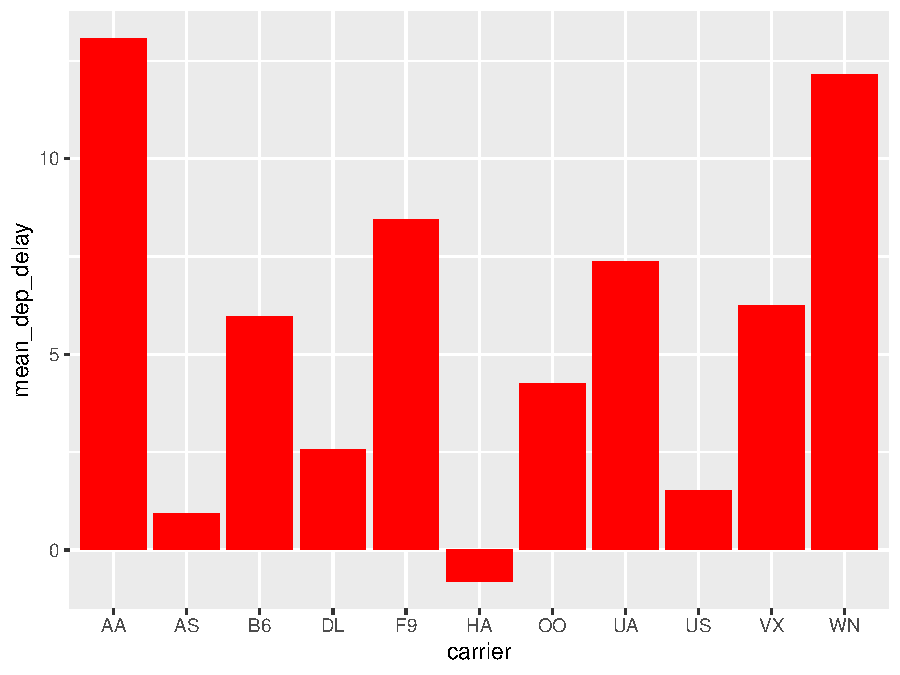
\includegraphics{thesis2_files/figure-latex/delaysboxplot-1.pdf}
\caption{\label{fig:delaysboxplot}Mean Delays by Airline}
\end{figure}
Here is a reference to this image: Figure \ref{fig:delaysboxplot}.

A table linking these carrier codes to airline names is available at \url{https://github.com/ismayc/pnwflights14/blob/master/data/airlines.csv}.

\clearpage

Next, we will explore the use of the \texttt{out.extra} chunk option, which can be used to shrink or expand an image loaded from a file by specifying \texttt{"scale=\ "}. Here we use the mathematical graph stored in the ``subdivision.pdf'' file.
\begin{figure}
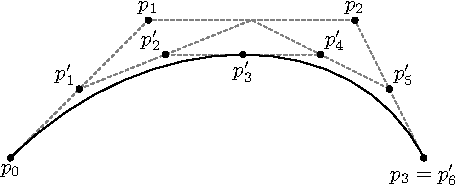
\includegraphics[scale=0.75]{figure/subdivision} \caption{Subdiv. graph}\label{fig:subd}
\end{figure}
Here is a reference to this image: Figure \ref{fig:subd}. Note that \texttt{echo=FALSE} is specified so that the \textbf{R} code is hidden in the document.

\textbf{More Figure Stuff}

Lastly, we will explore how to rotate and enlarge figures using the \texttt{out.extra} chunk option. (Currently this only works in the PDF version of the book.)
\begin{figure}
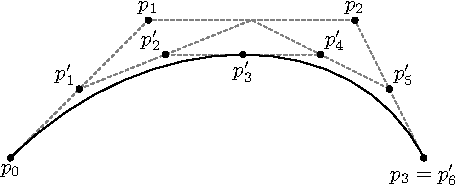
\includegraphics[angle=180, scale=1.1]{figure/subdivision} \caption{A Larger Figure, Flipped Upside Down}\label{fig:subd2}
\end{figure}
As another example, here is a reference: Figure \ref{fig:subd2}.

\hypertarget{footnotes-and-endnotes}{%
\section{Footnotes and Endnotes}\label{footnotes-and-endnotes}}

You might want to footnote something.\footnote{footnote text} The footnote will be in a smaller font and placed appropriately. Endnotes work in much the same way.

\hypertarget{bibliographies}{%
\section{Bibliographies}\label{bibliographies}}

Of course you will need to cite things, and you will probably accumulate an armful of sources. There are a variety of tools available for creating a bibliography database (stored with the .bib extension). In addition to BibTeX suggested below, you may want to consider using the free and easy-to-use tool called Zotero. Some Zotero documentation is at \url{http://libguides.reed.edu/citation/zotero}. In addition, a tutorial is available from Middlebury College at \url{http://sites.middlebury.edu/zoteromiddlebury/}.

\emph{R Markdown} uses \emph{pandoc} (\url{http://pandoc.org/}) to build its bibliographies. One nice caveat of this is that you won't have to do a second compile to load in references as standard LaTeX requires. To cite references in your thesis (after creating your bibliography database), place the reference name inside square brackets and precede it by the ``at'' symbol. For example, here's a reference to a book about worrying: {[}\protect\hyperlink{ref-Molina1994}{1}{]}. This \texttt{Molina1994} entry appears in a file called \texttt{thesis.bib} in the \texttt{bib} folder. This bibliography database file was created by a program called BibTeX. You can call this file something else if you like (look at the YAML header in the main .Rmd file) and, by default, is to placed in the \texttt{bib} folder.

For more information about BibTeX and bibliographies, see (\url{http://web.reed.edu/cis/help/latex/index.html})\footnote{\protect\hyperlink{ref-reedweb2007}{2}}. There are three pages on this topic: \emph{bibtex} (which talks about using BibTeX, at \url{http://web.reed.edu/cis/help/latex/bibtex.html}), \emph{bibtexstyles} (about how to find and use the bibliography style that best suits your needs, at \url{http://web.reed.edu/cis/help/latex/bibtexstyles.html}) and \emph{bibman} (which covers how to make and maintain a bibliography by hand, without BibTeX, at \url{http://web.reed.edu/cis/help/latex/bibman.html}). The last page will not be useful unless you have only a few sources.

If you look at the YAML header at the top of the main .Rmd file you can see that we can specify the style of the bibliography by referencing the appropriate csl file. You can download a variety of different style files at \url{https://www.zotero.org/styles}. Make sure to download the file into the csl folder.

\textbf{Tips for Bibliographies}
\begin{itemize}
\tightlist
\item
  Like with thesis formatting, the sooner you start compiling your bibliography for something as large as thesis, the better.
\item
  The cite key (a citation's label) needs to be unique from the other entries.
\item
  When you have more than one author or editor, you need to separate each author's name by the word ``and'' e.g.~\texttt{Author\ =\ \{Noble,\ Sam\ and\ Youngberg,\ Jessica\},}.
\item
  Bibliographies made using BibTeX (whether manually or using a manager) accept LaTeX markup, so you can italicize and add symbols as necessary.
\item
  To force capitalization in an article title or where all lowercase is generally used, bracket the capital letter in curly braces.
\end{itemize}
\hypertarget{anything-else}{%
\section{Anything else?}\label{anything-else}}

If you'd like to see examples of other things in this template, please \href{https://github.com/benmarwick/huskydown/issues/new}{contact us} (email \href{mailto:bmarwick@uw.edu}{\nolinkurl{bmarwick@uw.edu}}) with your suggestions. We love to see people using \emph{R Markdown} for their theses, and are happy to help.

\hypertarget{conclusion}{%
\chapter*{Conclusion}\label{conclusion}}
\addcontentsline{toc}{chapter}{Conclusion}

If we don't want Conclusion to have a chapter number next to it, we can add the \texttt{\{-\}} attribute.

\textbf{More info}

And here's some other random info: the first paragraph after a chapter title or section head \emph{shouldn't be} indented, because indents are to tell the reader that you're starting a new paragraph. Since that's obvious after a chapter or section title, proper typesetting doesn't add an indent there.

\appendix

\hypertarget{the-first-appendix}{%
\chapter{The First Appendix}\label{the-first-appendix}}

This first appendix includes all of the R chunks of code that were hidden throughout the document (using the \texttt{include\ =\ FALSE} chunk tag) to help with readibility and/or setup.

\textbf{In the main Rmd file}
\begin{Shaded}
\begin{Highlighting}[]
\CommentTok{# This chunk ensures that the gauchodown package is}
\CommentTok{# installed and loaded. This gauchodown package includes}
\CommentTok{# the template files for the thesis.}
\ControlFlowTok{if}\NormalTok{(}\OperatorTok{!}\KeywordTok{require}\NormalTok{(devtools))}
  \KeywordTok{install.packages}\NormalTok{(}\StringTok{"devtools"}\NormalTok{, }\DataTypeTok{repos =} \StringTok{"http://cran.rstudio.com"}\NormalTok{)}
\ControlFlowTok{if}\NormalTok{(}\OperatorTok{!}\KeywordTok{require}\NormalTok{(gauchodown))}
\NormalTok{  devtools}\OperatorTok{::}\KeywordTok{install_github}\NormalTok{(}\StringTok{"danovando/gauchodown"}\NormalTok{)}
\KeywordTok{library}\NormalTok{(gauchodown)}
\end{Highlighting}
\end{Shaded}
\textbf{In Chapter \ref{ref-labels}:}
\begin{Shaded}
\begin{Highlighting}[]
\CommentTok{# This chunk ensures that the huskydown package is}
\CommentTok{# installed and loaded. This huskydown package includes}
\CommentTok{# the template files for the thesis and also two functions}
\CommentTok{# used for labeling and referencing}
\ControlFlowTok{if}\NormalTok{(}\OperatorTok{!}\KeywordTok{require}\NormalTok{(devtools))}
  \KeywordTok{install.packages}\NormalTok{(}\StringTok{"devtools"}\NormalTok{, }\DataTypeTok{repos =} \StringTok{"http://cran.rstudio.com"}\NormalTok{)}
\ControlFlowTok{if}\NormalTok{(}\OperatorTok{!}\KeywordTok{require}\NormalTok{(dplyr))}
    \KeywordTok{install.packages}\NormalTok{(}\StringTok{"dplyr"}\NormalTok{, }\DataTypeTok{repos =} \StringTok{"http://cran.rstudio.com"}\NormalTok{)}
\ControlFlowTok{if}\NormalTok{(}\OperatorTok{!}\KeywordTok{require}\NormalTok{(ggplot2))}
    \KeywordTok{install.packages}\NormalTok{(}\StringTok{"ggplot2"}\NormalTok{, }\DataTypeTok{repos =} \StringTok{"http://cran.rstudio.com"}\NormalTok{)}
\ControlFlowTok{if}\NormalTok{(}\OperatorTok{!}\KeywordTok{require}\NormalTok{(ggplot2))}
    \KeywordTok{install.packages}\NormalTok{(}\StringTok{"bookdown"}\NormalTok{, }\DataTypeTok{repos =} \StringTok{"http://cran.rstudio.com"}\NormalTok{)}
\ControlFlowTok{if}\NormalTok{(}\OperatorTok{!}\KeywordTok{require}\NormalTok{(gauchodown))\{}
  \KeywordTok{library}\NormalTok{(devtools)}
\NormalTok{  devtools}\OperatorTok{::}\KeywordTok{install_github}\NormalTok{(}\StringTok{"benmarwick/gauchodown"}\NormalTok{)}
\NormalTok{  \}}
\KeywordTok{library}\NormalTok{(gauchodown)}
\NormalTok{flights <-}\StringTok{ }\KeywordTok{read.csv}\NormalTok{(}\StringTok{"data/flights.csv"}\NormalTok{)}
\end{Highlighting}
\end{Shaded}
\hypertarget{the-second-appendix-for-fun}{%
\chapter{The Second Appendix, for Fun}\label{the-second-appendix-for-fun}}

\hypertarget{colophon}{%
\chapter*{Colophon}\label{colophon}}
\addcontentsline{toc}{chapter}{Colophon}

This document is set in \href{https://github.com/georgd/EB-Garamond}{EB Garamond}, \href{https://github.com/adobe-fonts/source-code-pro/}{Source Code Pro} and \href{http://www.latofonts.com/lato-free-fonts/}{Lato}. The body text is set at 11pt with \(\familydefault\).

It was written in R Markdown and \(\LaTeX\), and rendered into PDF using \href{https://github.com/danovando/gauchodown}{gauchodown} and \href{https://github.com/rstudio/bookdown}{bookdown}.

This document was typeset using the XeTeX typesetting system, and the \href{http://staff.washington.edu/fox/tex/}{University of Washington Thesis class} class created by Jim Fox. Under the hood, the \href{https://github.com/UWIT-IAM/UWThesis}{University of Washington Thesis LaTeX template} is used to ensure that documents conform precisely to submission standards. Other elements of the document formatting source code have been taken from the \href{https://github.com/stevenpollack/ucbthesis}{Latex, Knitr, and RMarkdown templates for UC Berkeley's graduate thesis}, and \href{https://github.com/suchow/Dissertate}{Dissertate: a LaTeX dissertation template to support the production and typesetting of a PhD dissertation at Harvard, Princeton, and NYU}

The source files for this thesis, along with all the data files, have been organised into an R package, xxx, which is available at \url{https://github.com/xxx/xxx}. A hard copy of the thesis can be found in the University of Washington library.

This version of the thesis was generated on 2021-01-07 12:00:53. The repository is currently at this commit:

The computational environment that was used to generate this version is as follows:
\begin{verbatim}
- Session info ---------------------------------------------------------------
 setting  value                       
 version  R version 4.0.3 (2020-10-10)
 os       Windows 10 x64              
 system   x86_64, mingw32             
 ui       RTerm                       
 language (EN)                        
 collate  English_United States.1252  
 ctype    English_United States.1252  
 tz       Europe/Berlin               
 date     2021-01-07                  

- Packages -------------------------------------------------------------------
 package     * version date       lib source                               
 abind         1.4-5   2016-07-21 [1] CRAN (R 4.0.3)                       
 assertthat    0.2.1   2019-03-21 [1] CRAN (R 4.0.3)                       
 backports     1.2.0   2020-11-02 [1] CRAN (R 4.0.3)                       
 bookdown      0.21    2020-10-13 [1] CRAN (R 4.0.3)                       
 boot          1.3-25  2020-04-26 [2] CRAN (R 4.0.3)                       
 broom         0.7.3   2020-12-16 [1] CRAN (R 4.0.3)                       
 callr         3.5.1   2020-10-13 [1] CRAN (R 4.0.3)                       
 car           3.0-10  2020-09-29 [1] CRAN (R 4.0.3)                       
 carData       3.0-4   2020-05-22 [1] CRAN (R 4.0.3)                       
 cellranger    1.1.0   2016-07-27 [1] CRAN (R 4.0.3)                       
 cli           2.2.0   2020-11-20 [1] CRAN (R 4.0.3)                       
 colorspace    2.0-0   2020-11-11 [1] CRAN (R 4.0.3)                       
 cowplot     * 1.1.1   2020-12-30 [1] CRAN (R 4.0.3)                       
 crayon        1.3.4   2017-09-16 [1] CRAN (R 4.0.3)                       
 curl          4.3     2019-12-02 [1] CRAN (R 4.0.3)                       
 data.table    1.13.4  2020-12-08 [1] CRAN (R 4.0.3)                       
 DBI           1.1.0   2019-12-15 [1] CRAN (R 4.0.3)                       
 dbplyr        2.0.0   2020-11-03 [1] CRAN (R 4.0.3)                       
 desc          1.2.0   2018-05-01 [1] CRAN (R 4.0.3)                       
 devtools    * 2.3.2   2020-09-18 [1] CRAN (R 4.0.3)                       
 digest        0.6.27  2020-10-24 [1] CRAN (R 4.0.3)                       
 dplyr       * 1.0.2   2020-08-18 [1] CRAN (R 4.0.3)                       
 ellipsis      0.3.1   2020-05-15 [1] CRAN (R 4.0.3)                       
 evaluate      0.14    2019-05-28 [1] CRAN (R 4.0.3)                       
 fansi         0.4.1   2020-01-08 [1] CRAN (R 4.0.3)                       
 farver        2.0.3   2020-01-16 [1] CRAN (R 4.0.3)                       
 forcats     * 0.5.0   2020-03-01 [1] CRAN (R 4.0.3)                       
 foreign       0.8-81  2020-12-22 [2] CRAN (R 4.0.3)                       
 fs            1.5.0   2020-07-31 [1] CRAN (R 4.0.3)                       
 gauchodown  * 1.0     2021-01-07 [1] Github (danovando/gauchodown@d9a19b8)
 generics      0.1.0   2020-10-31 [1] CRAN (R 4.0.3)                       
 ggplot2     * 3.3.3   2020-12-30 [1] CRAN (R 4.0.3)                       
 ggpubr      * 0.4.0   2020-06-27 [1] CRAN (R 4.0.3)                       
 ggsci         2.9     2018-05-14 [1] CRAN (R 4.0.3)                       
 ggsignif      0.6.0   2019-08-08 [1] CRAN (R 4.0.3)                       
 git2r         0.27.1  2020-05-03 [1] CRAN (R 4.0.3)                       
 glue          1.4.2   2020-08-27 [1] CRAN (R 4.0.3)                       
 gtable        0.3.0   2019-03-25 [1] CRAN (R 4.0.3)                       
 haven         2.3.1   2020-06-01 [1] CRAN (R 4.0.3)                       
 highr         0.8     2019-03-20 [1] CRAN (R 4.0.3)                       
 hms           0.5.3   2020-01-08 [1] CRAN (R 4.0.3)                       
 htmltools     0.5.0   2020-06-16 [1] CRAN (R 4.0.3)                       
 httr          1.4.2   2020-07-20 [1] CRAN (R 4.0.3)                       
 jsonlite      1.7.2   2020-12-09 [1] CRAN (R 4.0.3)                       
 knitr       * 1.30    2020-09-22 [1] CRAN (R 4.0.3)                       
 labeling      0.4.2   2020-10-20 [1] CRAN (R 4.0.3)                       
 lattice       0.20-41 2020-04-02 [2] CRAN (R 4.0.3)                       
 lifecycle     0.2.0   2020-03-06 [1] CRAN (R 4.0.3)                       
 lme4        * 1.1-26  2020-12-01 [1] CRAN (R 4.0.3)                       
 lubridate     1.7.9.2 2020-11-13 [1] CRAN (R 4.0.3)                       
 magrittr      2.0.1   2020-11-17 [1] CRAN (R 4.0.3)                       
 MASS          7.3-53  2020-09-09 [2] CRAN (R 4.0.3)                       
 Matrix      * 1.2-18  2019-11-27 [2] CRAN (R 4.0.3)                       
 memoise       1.1.0   2017-04-21 [1] CRAN (R 4.0.3)                       
 minqa         1.2.4   2014-10-09 [1] CRAN (R 4.0.3)                       
 modelr        0.1.8   2020-05-19 [1] CRAN (R 4.0.3)                       
 munsell       0.5.0   2018-06-12 [1] CRAN (R 4.0.3)                       
 nlme        * 3.1-151 2020-12-10 [2] CRAN (R 4.0.3)                       
 nloptr        1.2.2.2 2020-07-02 [1] CRAN (R 4.0.3)                       
 openxlsx      4.2.3   2020-10-27 [1] CRAN (R 4.0.3)                       
 pillar        1.4.7   2020-11-20 [1] CRAN (R 4.0.3)                       
 pkgbuild      1.2.0   2020-12-15 [1] CRAN (R 4.0.3)                       
 pkgconfig     2.0.3   2019-09-22 [1] CRAN (R 4.0.3)                       
 pkgload       1.1.0   2020-05-29 [1] CRAN (R 4.0.3)                       
 plyr          1.8.6   2020-03-03 [1] CRAN (R 4.0.3)                       
 prettyunits   1.1.1   2020-01-24 [1] CRAN (R 4.0.3)                       
 processx      3.4.5   2020-11-30 [1] CRAN (R 4.0.3)                       
 ps            1.5.0   2020-12-05 [1] CRAN (R 4.0.3)                       
 purrr       * 0.3.4   2020-04-17 [1] CRAN (R 4.0.3)                       
 R6            2.5.0   2020-10-28 [1] CRAN (R 4.0.3)                       
 Rcpp          1.0.5   2020-07-06 [1] CRAN (R 4.0.3)                       
 readr       * 1.4.0   2020-10-05 [1] CRAN (R 4.0.3)                       
 readxl        1.3.1   2019-03-13 [1] CRAN (R 4.0.3)                       
 remotes       2.2.0   2020-07-21 [1] CRAN (R 4.0.3)                       
 reprex        0.3.0   2019-05-16 [1] CRAN (R 4.0.3)                       
 reshape2    * 1.4.4   2020-04-09 [1] CRAN (R 4.0.3)                       
 rio           0.5.16  2018-11-26 [1] CRAN (R 4.0.3)                       
 rlang         0.4.10  2020-12-30 [1] CRAN (R 4.0.3)                       
 rmarkdown     2.6     2020-12-14 [1] CRAN (R 4.0.3)                       
 rprojroot     2.0.2   2020-11-15 [1] CRAN (R 4.0.3)                       
 rstatix     * 0.6.0   2020-06-18 [1] CRAN (R 4.0.3)                       
 rstudioapi    0.13    2020-11-12 [1] CRAN (R 4.0.3)                       
 rvest         0.3.6   2020-07-25 [1] CRAN (R 4.0.3)                       
 scales        1.1.1   2020-05-11 [1] CRAN (R 4.0.3)                       
 sessioninfo   1.1.1   2018-11-05 [1] CRAN (R 4.0.3)                       
 statmod       1.4.35  2020-10-19 [1] CRAN (R 4.0.3)                       
 stringi       1.5.3   2020-09-09 [1] CRAN (R 4.0.3)                       
 stringr     * 1.4.0   2019-02-10 [1] CRAN (R 4.0.3)                       
 testthat      3.0.1   2020-12-17 [1] CRAN (R 4.0.3)                       
 tibble      * 3.0.4   2020-10-12 [1] CRAN (R 4.0.3)                       
 tidyr       * 1.1.2   2020-08-27 [1] CRAN (R 4.0.3)                       
 tidyselect    1.1.0   2020-05-11 [1] CRAN (R 4.0.3)                       
 tidyverse   * 1.3.0   2019-11-21 [1] CRAN (R 4.0.3)                       
 usethis     * 2.0.0   2020-12-10 [1] CRAN (R 4.0.3)                       
 utf8          1.1.4   2018-05-24 [1] CRAN (R 4.0.3)                       
 vctrs         0.3.6   2020-12-17 [1] CRAN (R 4.0.3)                       
 withr         2.3.0   2020-09-22 [1] CRAN (R 4.0.3)                       
 xfun          0.19    2020-10-30 [1] CRAN (R 4.0.3)                       
 xml2          1.3.2   2020-04-23 [1] CRAN (R 4.0.3)                       
 yaml          2.2.1   2020-02-01 [1] CRAN (R 4.0.3)                       
 zip           2.1.1   2020-08-27 [1] CRAN (R 4.0.3)                       

[1] D:/rlib
[2] D:/R/R-4.0.3/library
\end{verbatim}
\backmatter

\hypertarget{references}{%
\chapter*{References}\label{references}}
\addcontentsline{toc}{chapter}{References}

\markboth{References}{References}

\noindent

\setlength{\parindent}{-0.20in}
\setlength{\leftskip}{0.20in}
\setlength{\parskip}{8pt}

\hypertarget{refs}{}
\leavevmode\hypertarget{ref-Molina1994}{}%
{[}1{]} S. T. Molina and T. D. Borkovec, ``The Penn State worry questionnaire: Psychometric properties and associated characteristics,'' in \emph{Worrying: Perspectives on theory, assessment and treatment}, G. C. L. Davey and F. Tallis, Eds. New York: Wiley, 1994, pp. 265--283.

\leavevmode\hypertarget{ref-reedweb2007}{}%
{[}2{]} Reed~College, ``LaTeX your document.'' 2007 {[}Online{]}. Available: \url{http://web.reed.edu/cis/help/LaTeX/index.html}

\leavevmode\hypertarget{ref-angel2000}{}%
{[}3{]} E. Angel, \emph{Interactive computer graphics : A top-down approach with opengl}. Boston, MA: Addison Wesley Longman, 2000.

\leavevmode\hypertarget{ref-angel2001}{}%
{[}4{]} E. Angel, \emph{Batch-file computer graphics : A bottom-up approach with quicktime}. Boston, MA: Wesley Addison Longman, 2001.

\leavevmode\hypertarget{ref-angel2002a}{}%
{[}5{]} E. Angel, \emph{Test second book by angel}. Boston, MA: Wesley Addison Longman, 2001.

\end{ucmainmatter}
\end{document}

%---Set Headers and Footers ------------------------------------------------------
\pagestyle{fancy}
\renewcommand{\chaptermark}[1]{\markboth{{\sf #1 \hspace*{\fill} Chapter~\thechapter}}{} }
\renewcommand{\sectionmark}[1]{\markright{ {\sf Section~\thesection \hspace*{\fill} #1 }}}
\fancyhf{}

\makeatletter \if@twoside \fancyhead[LO]{\small \rightmark} \fancyhead[RE]{\small\leftmark} \else \fancyhead[LO]{\small\leftmark}
\fancyhead[RE]{\small\rightmark} \fi

\def\cleardoublepage{\clearpage\if@openright \ifodd\c@page\else
  \hbox{}
  \vspace*{\fill}
  \begin{center}
    This page intentionally left blank
  \end{center}
  \vspace{\fill}
  \thispagestyle{plain}
  \newpage
  \fi \fi}
\makeatother
\fancyfoot[c]{\textrm{\textup{\thepage}}} % page number
\fancyfoot[C]{\thepage}
\renewcommand{\headrulewidth}{0.4pt}

\fancypagestyle{plain} { \fancyhf{} \fancyfoot[C]{\thepage}
\renewcommand{\headrulewidth}{0pt}
\renewcommand{\footrulewidth}{0pt}}

